\documentclass[11pt,a4paper]{article}

% --- Core Packages ---
\usepackage[utf8]{inputenc}
\usepackage[T1]{fontenc}
\usepackage[margin=2.2cm,top=2.5cm,bottom=2.5cm]{geometry}
\usepackage{amsmath,amssymb,amsfonts}
\usepackage{graphicx}
\usepackage{booktabs}
\usepackage{tabularx}
\usepackage{array}
\usepackage{xcolor}
\usepackage{tikz}
\usetikzlibrary{shapes,arrows.meta,positioning,fit,backgrounds,calc}
\usepackage{fancyhdr}
\usepackage{enumitem}
\usepackage{microtype}
\usepackage{titlesec}
\usepackage{caption}

\usepackage[hidelinks]{hyperref}

% --- Section Styling ---
\titleformat{\section}{\normalfont\Large\bfseries}{\thesection}{0.8em}{}
\titleformat{\subsection}{\normalfont\large\bfseries}{\thesubsection}{0.8em}{}
\titleformat{\subsubsection}{\normalfont\normalsize\bfseries}{\thesubsubsection}{0.8em}{}

\titlespacing*{\section}{0pt}{1.8ex plus 0.5ex minus 0.2ex}{1.2ex plus 0.2ex}
\titlespacing*{\subsection}{0pt}{1.5ex plus 0.4ex minus 0.2ex}{0.8ex plus 0.2ex}
\titlespacing*{\subsubsection}{0pt}{1.2ex plus 0.3ex minus 0.2ex}{0.6ex plus 0.2ex}

% --- Header and Footer ---
\pagestyle{fancy}
\fancyhf{}
\renewcommand{\headrulewidth}{0pt}
\renewcommand{\footrulewidth}{0pt}
\fancyfoot[C]{\small\thepage}

% --- Caption Styling (Clean, Normal Weight) ---
\captionsetup{font=small,labelfont=normalfont,textfont=normalfont,margin=10pt}

% ==============================================================================
% DOCUMENT BODY
% ==============================================================================
\begin{document}

% --- Title Block ---
\begin{center}
  {\LARGE \textbf{Autonomous Agile Aerobatics on a Crazyflie Quadcopter via Reinforcement Learning and On-Device Inference}} \\[0.7em]
  {\large Technical Project Report for the 5th AI-Hub Artificial Intelligence Competition (2026)} \\[0.3em]
  {\normalsize University of Patras, Greece} \\[1.0em]
  
  Andreas Panagopoulos \\[0.2em]
  Department of Electrical and Computer Engineering, University of Patras, Greece \\
  \texttt{andreas.panagopoulos@ac.upatras.gr} \\[1.0em]
\end{center}

\vspace{0.2em}

% --- Abstract ---
\begin{abstract}
Executing fast, acrobatic flight manoeuvres, such as complete 360-degree power flips, on autonomous micro drones is an enduring problem in robotics and control. Small quadcopters like the Bitcraze Crazyflie 2.1 have high thrust to weight potential, but their real-time performance is tightly constrained by limited onboard computing, rapid battery voltage drops during peak throttle, aerodynamic disturbances during inversion, and optical tracking occlusions. 

This report presents an autonomous flight control pipeline that performs acrobatic flips directly onboard the quadcopter in real time. An asymmetric actor-critic policy was trained with proximal policy optimization inside a parallelized JAX and MuJoCo simulation environment executing thousands of steps per second. Training decouples a large privileged critic that observes hidden simulation states from a compact neural network actor with thirty-two hidden units. To overcome the reality gap between simulation and the real vehicle, a lightweight recurrent history encoder with gated recurrent units converts sequences of noisy sensor readings into a sixteen-dimensional latent state. This latent state acts as an implicit system identifier, capturing motor delay, unmodeled drag, and battery degradation without requiring explicit mathematical parameter estimation during flight.

The policy compiles to native C code through the ST Edge AI toolchain, running deterministically at 100\,Hz inside a FreeRTOS controller task with sub-millisecond execution latency on an ARM Cortex-M4 microcontroller. The policy commands an onboard 1\,kHz rate PID stabilizer. To ensure hardware safety, an estimator plausibility filter prevents optical tracking losses from generating runaway position estimates, supported by a smooth failsafe descent mode. Hardware flight tests confirm that the quadcopter performs autonomous flips with vertical climb clearance, rapid inversion, and upright recovery without human intervention or external computers. Furthermore, the latent representation allowed the controller to fly an upgraded motor setup without retraining the policy.
\end{abstract}

\vspace{0.4em}
\noindent\textit{Keywords:} Micro aerial vehicles, deep reinforcement learning, asymmetric actor-critic, sim-to-real transfer, embedded edge intelligence, on-device neural inference.

\vspace{0.8em}

% ==============================================================================
% SECTION 1: INTRODUCTION
% ==============================================================================
\section{Introduction and Project Goals}
\label{sec:introduction}

Micro quadcopters in the sub-50 gram weight class, such as the open-source Bitcraze Crazyflie 2.1 (Figure~\ref{fig:hardware_platform}a), provide high maneuverability, mechanical compliance, and safe indoor operation. These small drones are well suited for exploring confined indoor environments and complex spaces. Performing aggressive manoeuvres, such as complete 360-degree flips, presents an interesting technical challenge in agile flight control under tight physical constraints.

However, performing agile aerobatics on micro-scale quadcopters involves severe engineering constraints that do not arise on larger multi-rotor drones:

First, onboard computing resources are severely limited. Full-scale drones carry multi-core processors drawing significant battery power. In contrast, micro quadcopters must operate within a strict payload budget of less than fifteen grams. The entire computation runs on a single low-power microcontroller, the STM32F405, featuring an ARM Cortex-M4 core at 168\,MHz with 192\,KB of RAM and 1024\,KB of Flash memory. This microcontroller must simultaneously handle real-time operating system tasks, radio communication, Kalman state estimation, and motor speed generation.

Second, aggressive flight regimes create substantial aerodynamic and actuator discrepancies between simulation and reality. Fast manoeuvres expose the drone to nonlinear aerodynamic effects, including blade flapping, turbulent rotor wake interactions, and rapid battery voltage drops. When demanding full throttle during a vertical climb, the single-cell lithium polymer battery experiences voltage sag, dropping available motor thrust significantly. Conventional cascaded linear controllers fail under these saturated and coupled flight conditions.

Third, optical tracking dropouts cause state runaway. In indoor optical positioning environments using Lighthouse v2 tracking, inverted flight causes the optical sensors on the top deck of the vehicle (Figure~\ref{fig:hardware_platform}b) to lose line of sight to the base stations. During such occlusions, the onboard extended Kalman filter integrates sensor noise and gravity misalignments, which can cause estimated altitude to drift rapidly into unphysical values. A controller that trusts this false altitude reading will abruptly cut motor thrust and crash.

\begin{figure}[t!]
  \centering
  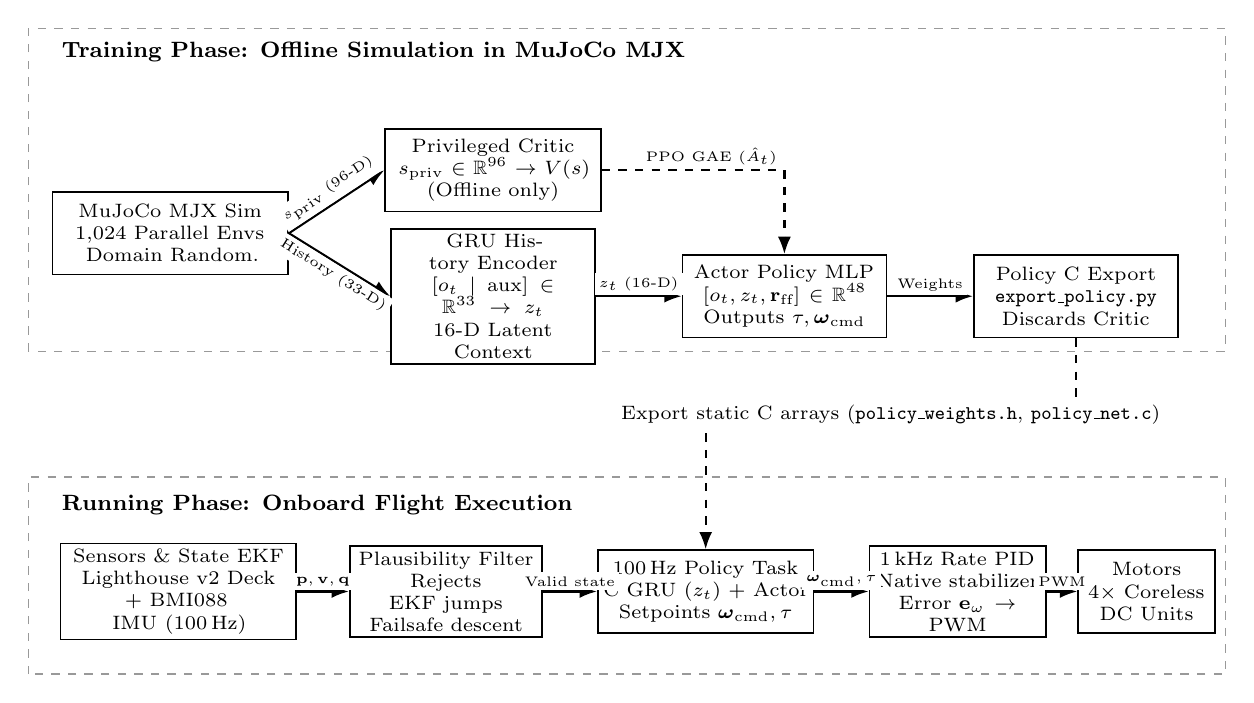
\begin{tikzpicture}[
    block/.style={rectangle, draw=black, line width=0.6pt, fill=white, text width=2.45cm, align=center, minimum height=1.05cm, font=\scriptsize, inner sep=2pt},
    wideblock/.style={rectangle, draw=black, line width=0.6pt, fill=white, text width=2.85cm, align=center, minimum height=1.05cm, font=\scriptsize, inner sep=2pt},
    arrow/.style={-{Latex[length=2.2mm]}, thick, black},
    darrow/.style={-{Latex[length=2.2mm]}, thick, dashed, black},
    lbl/.style={fill=white, inner sep=1.5pt, font=\tiny, align=center}
  ]
    % --- TRAINING PHASE PANEL ---
    \draw[draw=black!40, dashed, line width=0.6pt] (-7.6, 0.3) rectangle (7.6, 4.4);
    \node[font=\footnotesize\bfseries, anchor=west] at (-7.3, 4.1) {Training Phase: Offline Simulation in MuJoCo MJX};

    \node[wideblock] (sim) at (-5.8, 1.8) {MuJoCo MJX Sim\\ 1,024 Parallel Envs\\ Domain Random.};
    \node[block, text width=2.6cm] (critic) at (-1.7, 2.6) {Privileged Critic\\ $s_{\text{priv}} \in \mathbb{R}^{96} \to V(s)$\\ \scriptsize (Offline only)};
    \node[block] (gru) at (-1.7, 1.0) {GRU History Encoder\\ $[o_t \mid \text{aux}] \in \mathbb{R}^{33} \to z_t$\\ \scriptsize 16-D Latent Context};
    \node[block] (actor) at (2.0, 1.0) {Actor Policy MLP\\ $[o_t, z_t, \mathbf{r}_{\text{ff}}] \in \mathbb{R}^{48}$\\ Outputs $\tau, \boldsymbol{\omega}_{\text{cmd}}$};
    \node[block] (export) at (5.7, 1.0) {Policy C Export\\ \texttt{export\_policy.py}\\ Discards Critic};

    \draw[arrow] (sim.east) -- (critic.west) node[midway, lbl, sloped, above] {$s_{\text{priv}}$ (96-D)};
    \draw[arrow] (sim.east) -- (gru.west) node[midway, lbl, sloped, below] {History (33-D)};
    \draw[arrow] (gru) -- node[lbl, above] {$z_t$ (16-D)} (actor);
    \draw[darrow] (critic.east) -| node[lbl, pos=0.3, above] {PPO GAE ($\hat{A}_t$)} (actor.north);
    \draw[arrow] (actor) -- node[lbl, above] {Weights} (export);

    % --- RUNNING / DEPLOYMENT PHASE PANEL ---
    \draw[draw=black!40, dashed, line width=0.6pt] (-7.6, -3.8) rectangle (7.6, -1.3);
    \node[font=\footnotesize\bfseries, anchor=west] at (-7.3, -1.65) {Running Phase: Onboard Flight Execution};

    \node[wideblock] (sensors) at (-5.7, -2.75) {Sensors \& State EKF\\ Lighthouse v2 Deck\\ + BMI088 IMU (100\,Hz)};
    \node[block, text width=2.3cm] (guard) at (-2.3, -2.75) {Plausibility Filter\\ Rejects EKF jumps\\ Failsafe descent};
    \node[block, text width=2.6cm] (policy) at (1.0, -2.75) {100\,Hz Policy Task\\ C GRU ($z_t$) + Actor\\ Setpoints $\boldsymbol{\omega}_{\text{cmd}}, \tau$};
    \node[block, text width=2.1cm] (pid) at (4.2, -2.75) {1\,kHz Rate PID\\ Native stabilizer\\ Error $\mathbf{e}_\omega \to$ PWM};
    \node[block, text width=1.6cm] (motors) at (6.6, -2.75) {Motors\\ 4$\times$ Coreless\\ DC Units};

    \draw[arrow] (sensors) -- node[lbl, above] {$\mathbf{p}, \mathbf{v}, \mathbf{q}$} (guard);
    \draw[arrow] (guard) -- node[lbl, above] {Valid state} (policy);
    \draw[arrow] (policy) -- node[lbl, above] {$\boldsymbol{\omega}_{\text{cmd}}, \tau$} (pid);
    \draw[arrow] (pid) -- node[lbl, above] {PWM} (motors);

    % --- LINK FROM TRAINING TO RUNNING ---
    \draw[darrow] (export.south) -- (5.7, -0.5) -- node[midway, fill=white, inner sep=2pt, font=\scriptsize] {Export static C arrays (\texttt{policy\_weights.h}, \texttt{policy\_net.c})} (1.0, -0.5) -- (policy.north);
  \end{tikzpicture}
  \caption{System architecture separated into offline training and onboard running phases. During training, 1,024 parallel environments in MuJoCo MJX optimize an asymmetric actor-critic policy and a recurrent history encoder. The policy export script converts the actor and frozen GRU into static C arrays. During physical flight, the C policy executes at 100\,Hz inside FreeRTOS on the STM32F405 microcontroller, validating state estimates through the plausibility filter and commanding angular rate setpoints to the native 1\,kHz Rate PID stabilizer.}
  \label{fig:system_overview}
\end{figure}

Figure~\ref{fig:system_overview} illustrates the end-to-end architecture separated into offline training and onboard running phases. To address these challenges, this project implements a unified reinforcement learning and embedded software pipeline with several key outcomes:
\begin{itemize}[leftmargin=*,itemsep=2pt]
  \item Autonomous aerobatic flight executed entirely on an onboard microcontroller without offboard computation or ground control loops.
  \item Real-time adaptation through a recurrent history encoder that maps noisy sensor sequences to a compact latent vector, compensating for battery discharge and motor differences.
  \item Accelerated simulation in MuJoCo MJX running thousands of parallel steps per second, allowing complete policy optimization in a few hours on standard workstation hardware.
  \item Practical firmware precautions with an estimator plausibility filter that saves the drone from crashing occasionally during optical tracking dropouts.
\end{itemize}

% ==============================================================================
% SECTION 2: DYNAMICS & SINGULARITY AVOIDANCE
% ==============================================================================
\section{Quadcopter Dynamics and Singularity Avoidance}
\label{sec:dynamics}

\begin{figure}[t!]
  \centering
  \begin{minipage}[b]{0.35\textwidth}
    \centering
    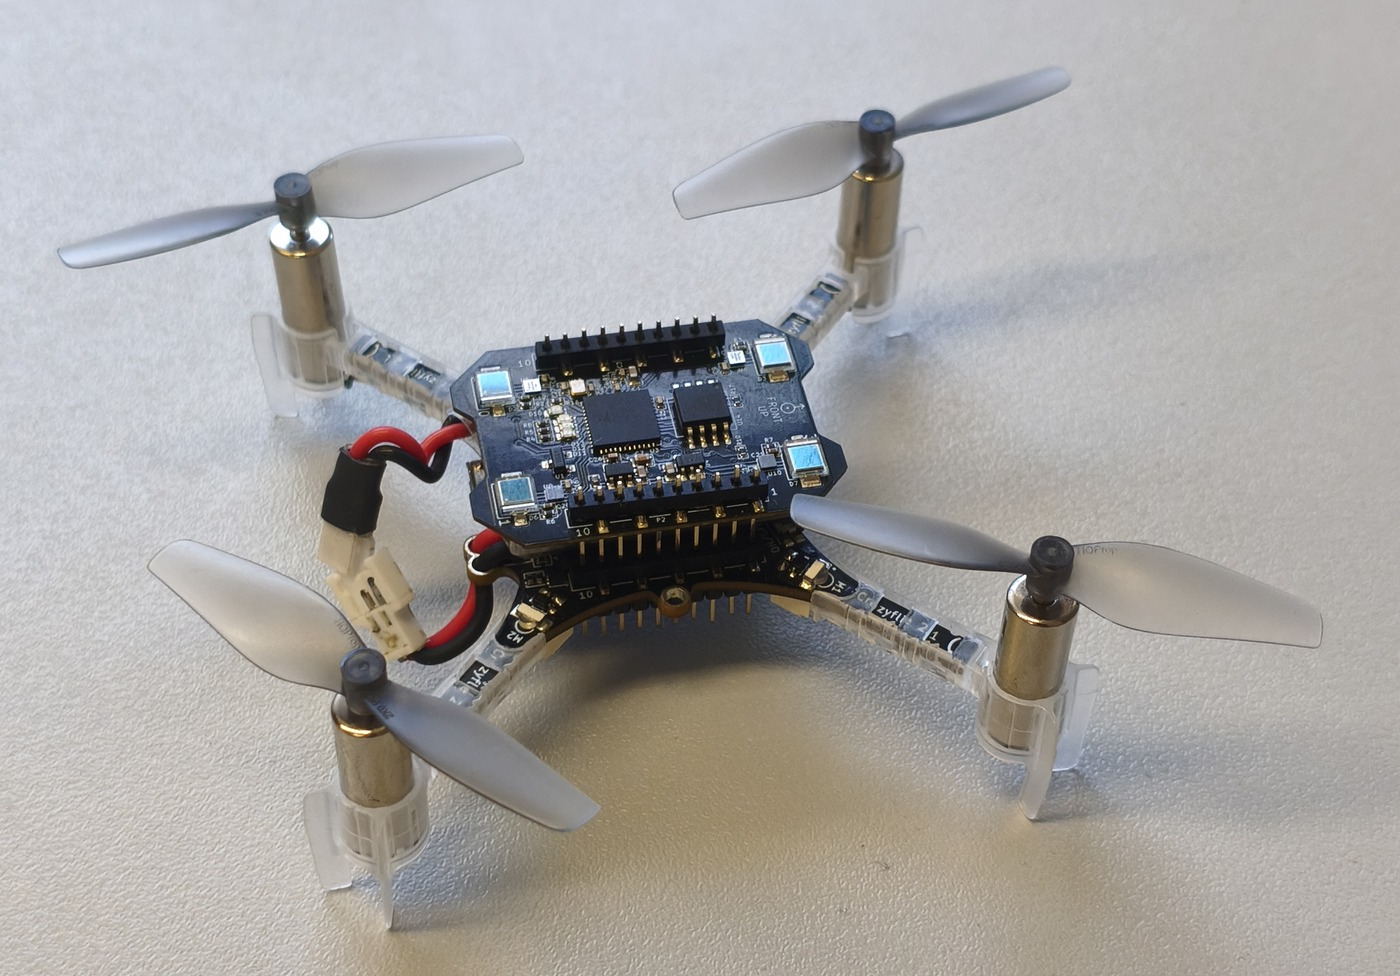
\includegraphics[width=\textwidth,height=3.8cm,keepaspectratio]{figures/crazyflie_hardware.jpg}
    \vspace{0.2em}
    \caption*{\footnotesize (a) Crazyflie 2.1 quadcopter}
  \end{minipage}
  \hfill
  \begin{minipage}[b]{0.30\textwidth}
    \centering
    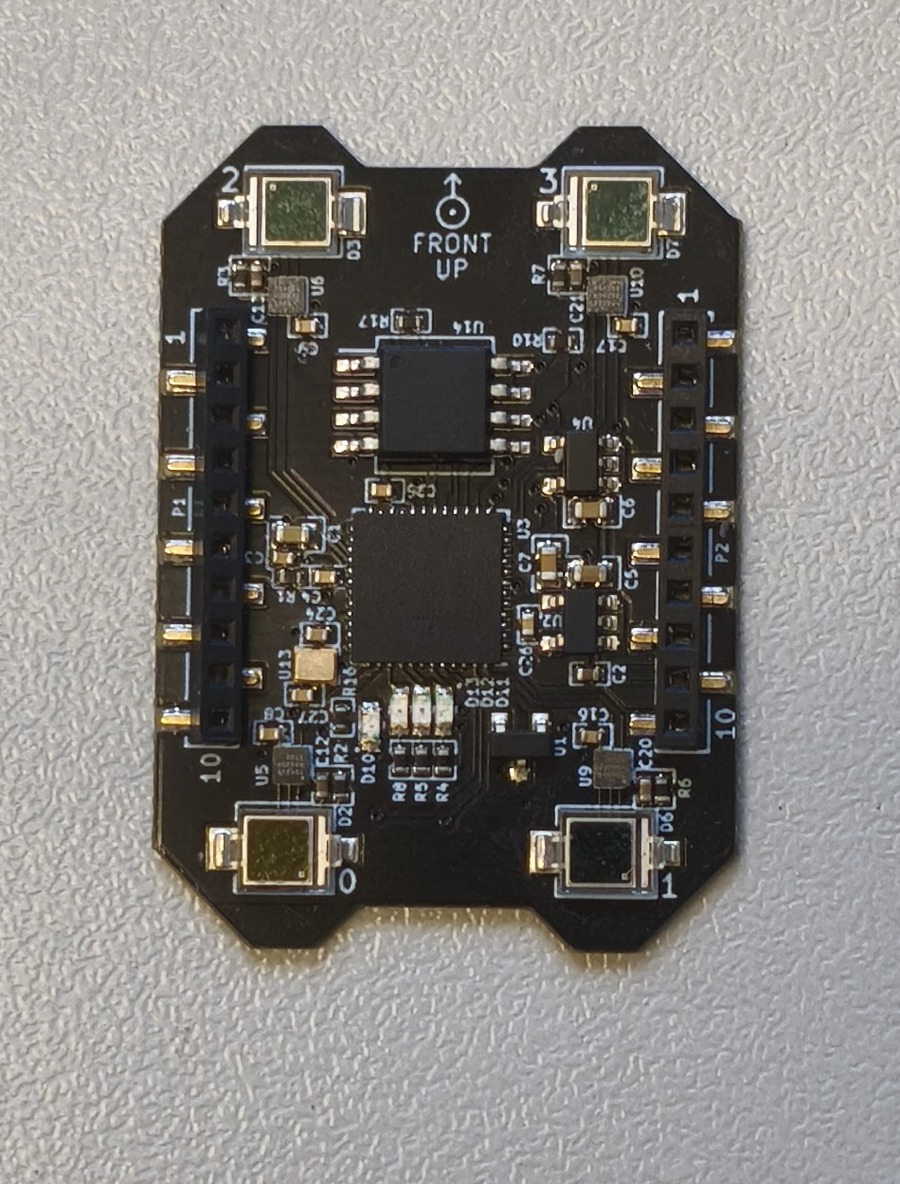
\includegraphics[width=\textwidth,height=3.8cm,keepaspectratio]{figures/lighthouse_deck.jpg}
    \vspace{0.2em}
    \caption*{\footnotesize (b) Lighthouse v2 deck}
  \end{minipage}
  \hfill
  \begin{minipage}[b]{0.30\textwidth}
    \centering
    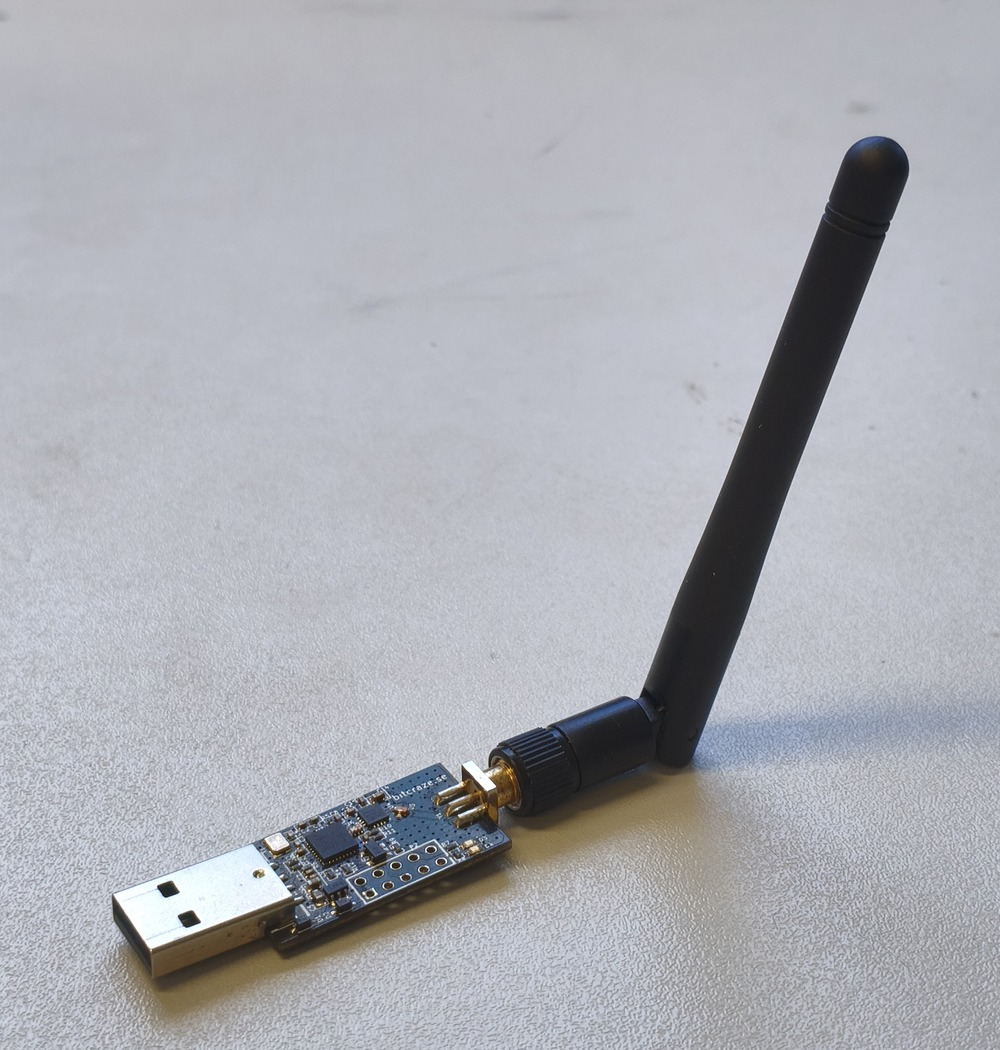
\includegraphics[width=\textwidth,height=3.8cm,keepaspectratio]{figures/crazyradio_dongle.jpg}
    \vspace{0.2em}
    \caption*{\footnotesize (c) Crazyradio dongle}
  \end{minipage}
  \vspace{-0.3em}
  \caption{Experimental micro quadcopter avionics and telemetry hardware. (a) Bitcraze Crazyflie 2.1 nano-quadcopter equipped with coreless DC motors, an onboard IMU, and an STM32F405 microcontroller. (b) Lighthouse optical receiver deck featuring four corner photodiodes (sensors 0--3) used to decode sweep angles from base station sweeps. (c) 2.4\,GHz Crazyradio PA USB dongle with external antenna for ground telemetry logging.}
  \label{fig:hardware_platform}
\end{figure}

\subsection{Equations of Motion}
The quadcopter is modeled as a 6-DOF rigid body with mass $m$ and diagonal inertia tensor $\mathbf{I} = \text{diag}(I_{xx}, I_{yy}, I_{zz})$ in an inertial coordinate frame. The state vector is defined as:
\begin{equation}
  \mathbf{s} = [\mathbf{p}^T, \mathbf{v}^T, \mathbf{q}^T, \boldsymbol{\omega}^T]^T \in \mathbb{R}^{13}
\end{equation}
where $\mathbf{p} = [x, y, z]^T$ denotes inertial position, $\mathbf{v} = [v_x, v_y, v_z]^T$ is linear velocity, $\mathbf{q} = [q_w, q_x, q_y, q_z]^T$ is the unit attitude quaternion, and $\boldsymbol{\omega} = [p, q, r]^T$ is the body angular velocity. The rigid-body equations of motion are given by:
\begin{align}
  \dot{\mathbf{p}} &= \mathbf{v} \label{eq:pos_dot} \\
  m \dot{\mathbf{v}} &= m \mathbf{g} + \mathbf{R}(\mathbf{q}) \mathbf{T}_B - \mathbf{D}_v \mathbf{v} \label{eq:vel_dot} \\
  \dot{\mathbf{q}} &= \frac{1}{2} \mathbf{q} \otimes \begin{bmatrix} 0 \\ \boldsymbol{\omega} \end{bmatrix} \label{eq:quat_dot} \\
  \mathbf{I} \dot{\boldsymbol{\omega}} &= \boldsymbol{\tau}_B - \boldsymbol{\omega} \times (\mathbf{I} \boldsymbol{\omega}) - \boldsymbol{\tau}_{\text{gyro}} \label{eq:omega_dot}
\end{align}
where $\mathbf{R}(\mathbf{q})$ transforms vectors from the body frame to the world frame, $\mathbf{g} = [0, 0, -9.81]^T\,\text{m/s}^2$ is gravitational acceleration, $\mathbf{D}_v$ is a linear aerodynamic drag tensor, and $\boldsymbol{\tau}_{\text{gyro}}$ accounts for rotor gyroscopic effects during rapid body rotations. Collective thrust $\mathbf{T}_B = [0, 0, T_{\text{total}}]^T$ and body moments $\boldsymbol{\tau}_B = [\tau_x, \tau_y, \tau_z]^T$ are generated by four rotors in an X configuration:
\begin{equation}
  \begin{bmatrix} T_{\text{total}} \\ \tau_x \\ \tau_y \\ \tau_z \end{bmatrix} =
  \begin{bmatrix}
    k_{Th} & k_{Th} & k_{Th} & k_{Th} \\
    -d_y k_{Th} & d_y k_{Th} & d_y k_{Th} & -d_y k_{Th} \\
    -d_x k_{Th} & -d_x k_{Th} & d_x k_{Th} & d_x k_{Th} \\
    -k_Q & k_Q & -k_Q & k_Q
  \end{bmatrix}
  \begin{bmatrix} \omega_{M1}^2 \\ \omega_{M2}^2 \\ \omega_{M3}^2 \\ \omega_{M4}^2 \end{bmatrix}
\end{equation}
where $d_x = d_y = 0.0325$\,m is the rotor arm distance from the center of mass, $k_{Th}$ is the rotor thrust factor, and $k_Q$ is the rotor reaction torque constant.

\subsection{Singularity Free Attitude Representation}
Standard flight controllers often parameterize orientation with Euler angles roll $\phi$, pitch $\theta$, and yaw $\psi$. However, Euler angle representations suffer from mathematical singularities during inverted aerobatics. The kinematic transformation between Euler angle rates and body angular velocities contains terms proportional to $\tan(\theta)$ and $1/\cos(\theta)$.

During a 360-degree pitch flip, the pitch angle rotates through $\pm 90^\circ$ and passes into full inversion at $180^\circ$. At $\pm 90^\circ$, Euler kinematics experience gimbal lock, causing numerical integration to diverge. In addition, when passing through complete inversion, roll and yaw angles jump discontinuously by $180^\circ$. These angle discontinuities inject massive artificial gradients into neural policy optimization.

To maintain mathematical continuity across all orientations, the system exclusively uses unit quaternions $\mathbf{q} \in \mathbb{S}^3$ throughout state estimation, reward calculation, and reference tracking. Orientation error is computed via quaternion conjugate multiplication:
\begin{equation}
  \mathbf{q}_{\text{err}} = \mathbf{q}_{\text{ref}}^* \otimes \mathbf{q} = \begin{bmatrix} q_{w,\text{err}} \\ \mathbf{q}_{v,\text{err}} \end{bmatrix}
\end{equation}
The policy observes the vector component $\mathbf{q}_{v,\text{err}} = [q_{x,\text{err}}, q_{y,\text{err}}, q_{z,\text{err}}]^T$, which remains continuous and smooth over the entire rotation space.

\subsection{Actuator Lag and Motor Hardware Configuration}
Coreless DC motors exhibit mechanical and electrical time constants that create first-order response lag:
\begin{equation}
  \dot{\omega}_{M,i} = \frac{1}{\tau} \left(\omega_{M,i}^{\text{cmd}} - \omega_{M,i}\right)
\end{equation}
with an effective time constant $\tau \approx 25$\,ms. When executing an aerobatic flip with body rates reaching 20\,rad/s, this delay produces an angular phase lag of roughly 28 degrees. Ignoring motor lag during training leads to severe over-rotation and crashes during real flight.

\begin{table}[t!]
  \centering
  \small
  \caption{Quadcopter avionics architecture and physical plant parameters across baseline and upgraded configurations.}
  \label{tab:hardware_specs}
  \begin{tabularx}{\textwidth}{>{\raggedright\arraybackslash}p{4.2cm}>{\raggedright\arraybackslash}X>{\raggedright\arraybackslash}X}
    \toprule
    Subsystem / Parameter & Baseline Configuration & Upgraded Aerobatic Configuration \\
    \midrule
    Flight Microcontroller & STM32F405 (ARM Cortex-M4, 168\,MHz) & STM32F405 (ARM Cortex-M4, 168\,MHz) \\
    Onboard Memory & 192\,KB RAM, 1024\,KB Flash & 192\,KB RAM, 1024\,KB Flash \\
    Inertial Measurement Unit & BMI088 (1\,kHz gyroscope feedback) & BMI088 (1\,kHz gyroscope feedback) \\
    Positioning System & Lighthouse v2 optical receiver deck & Lighthouse v2 optical receiver deck \\
    Real-Time Executive & FreeRTOS (two-rate architecture) & FreeRTOS (two-rate architecture) \\
    Motor Propulsion Units & 16\,mm coreless brushed DC motors & 20\,mm coreless brushed DC motors \\
    All-Up Flight Mass & 33\,g (nominal baseline airframe) & 41\,g (reinforced airframe) \\
    Maximum Total Thrust & 0.60\,N (4$\times$ 0.15\,N) & 1.19\,N (4$\times$ 0.30\,N) \\
    Thrust-to-Weight Ratio & 1.85 (marginal recovery headroom) & 2.97 (sufficient to arrest descent) \\
    \bottomrule
  \end{tabularx}
\end{table}

\begin{figure}[t!]
  \centering
  \begin{minipage}[b]{0.50\textwidth}
    \centering
    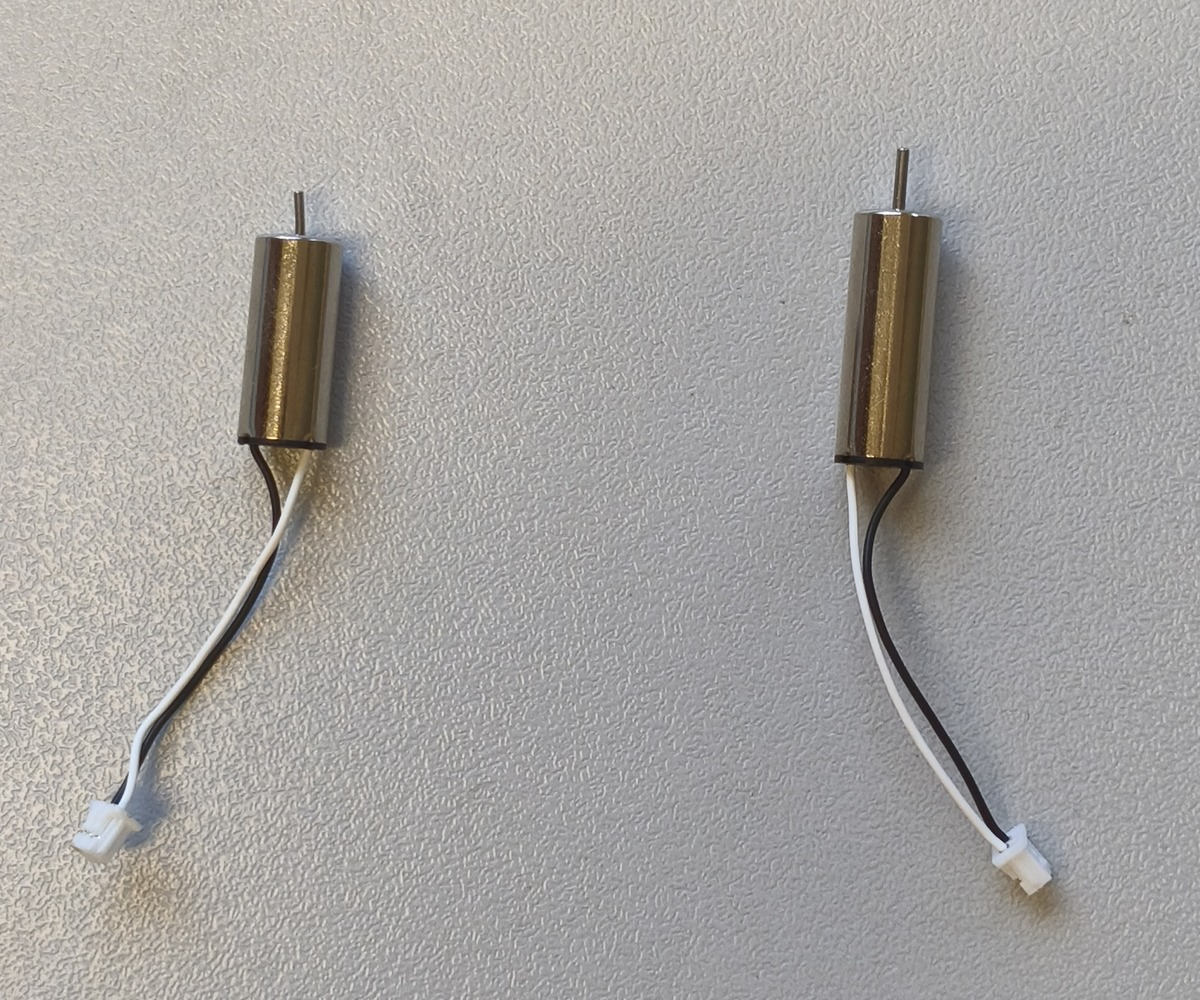
\includegraphics[width=\textwidth,height=4.4cm,keepaspectratio]{figures/motors_16mm_vs_20mm.jpg}
    \vspace{0.2em}
    \caption*{\footnotesize (a) Stock 16\,mm vs. upgraded 20\,mm motor}
  \end{minipage}
  \hfill
  \begin{minipage}[b]{0.45\textwidth}
    \centering
    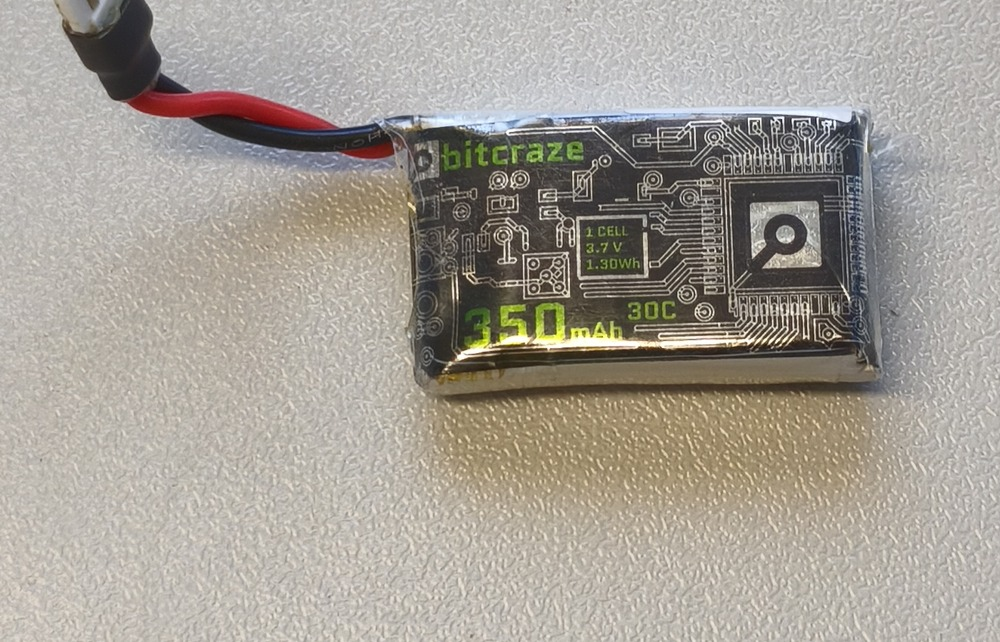
\includegraphics[width=\textwidth,height=4.4cm,keepaspectratio]{figures/lipo_battery.jpg}
    \vspace{0.2em}
    \caption*{\footnotesize (b) Single-cell 350\,mAh LiPo battery}
  \end{minipage}
  \vspace{-0.3em}
  \caption{Propulsion and power hardware components. (a) Physical comparison of the baseline 16\,mm coreless DC motor (left) against the upgraded 20\,mm high-thrust motor (right). (b) Single-cell 350\,mAh lithium-polymer flight battery subject to voltage sag during full-throttle bursts.}
  \label{fig:motors_battery}
\end{figure}

The physical vehicle was tested across two configurations, summarized in Table~\ref{tab:hardware_specs} and shown in Figure~\ref{fig:motors_battery}. The stock platform used 16\,mm motors with an all-up mass of 33\,g and a peak thrust of 0.60\,N, yielding a thrust-to-weight ratio of 1.85. Under this baseline, a vertical climb required over 90 percent throttle, leaving minimal control headroom to catch the vehicle after inversion. Upgraded 20\,mm motors were subsequently installed on the platform, increasing mass to 41\,g while raising maximum thrust to 1.19\,N, which raised the thrust-to-weight ratio to 2.97. The recurrent latent encoder absorbed this physical plant modification without retraining.

% ==============================================================================
% SECTION 3: MANOEUVRE DESIGN & FLIP PHASES
% ==============================================================================
\section{Manoeuvre Library and Trajectory Design}
\label{sec:trajectories}

\subsection{Trajectory Families}
To produce a robust policy capable of precise tracking and dynamic agility, an analytic reference trajectory suite was developed covering seven distinct flight regimes:
\begin{itemize}[leftmargin=*,itemsep=2pt]
  \item Precision hover: position regulation at target 3D spatial coordinates.
  \item 3D polynomial waypoints: smooth polynomial spline paths connecting sequential target points.
  \item Lemniscate figure-eight: planar and inclined figure-eight paths generated by harmonic curves.
  \item Vertical figure-eight: aggressive figure-eight trajectories oriented in a vertical plane with four times higher vertical acceleration demands.
  \item Slalom weave: lateral evasive flight patterns featuring rapid roll rate reversals.
  \item 3D orbit: circular trajectories with continuous orientation alignment along the velocity vector.
  \item Lissajous curves: coupled spatial curves that simultaneously excite pitch, roll, and yaw dynamics.
\end{itemize}

Every continuous reference trajectory incorporates a smooth quintic settle envelope:
\begin{equation}
  e(t) = 10\left(\frac{t}{T}\right)^3 - 15\left(\frac{t}{T}\right)^4 + 6\left(\frac{t}{T}\right)^5
\end{equation}
which smoothly drives tracking errors, velocity setpoints, and acceleration setpoints to zero at the end of the manoeuvre, ensuring a seamless handover to stationary hover. All trajectories are validated against a 1.5\,m by 1.5\,m safety footprint suited to the indoor flight volume.

\begin{figure}[t!]
  \centering
  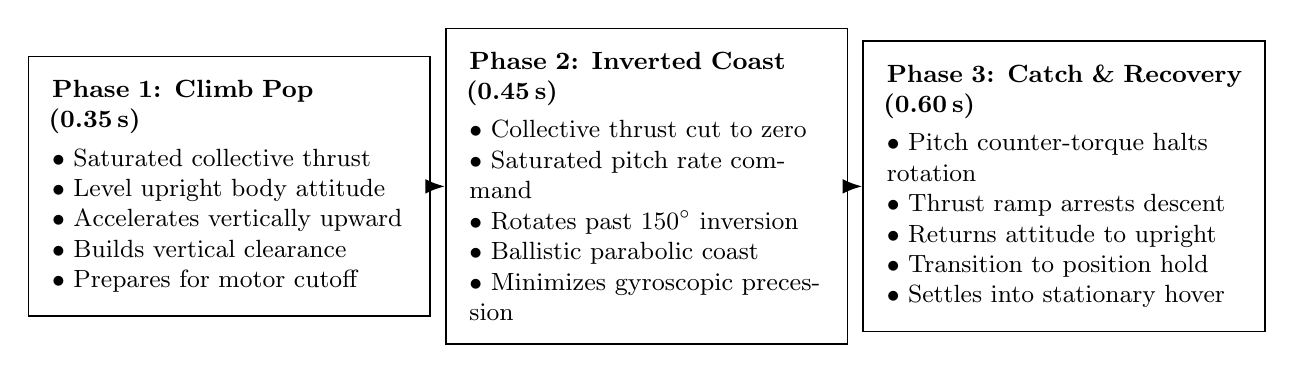
\begin{tikzpicture}[
    phasebox/.style={rectangle, draw=black, line width=0.6pt, fill=white, text width=4.5cm, minimum height=2.8cm, align=left, font=\small, inner sep=3mm},
    parrow/.style={-{Latex[length=2.5mm]}, thick, black}
  ]
    \node[phasebox] (p1) at (-5.3, 0) {
      \textbf{Phase 1: Climb Pop (0.35\,s)}\\[0.3em]
      $\bullet$ Saturated collective thrust\\
      $\bullet$ Level upright body attitude\\
      $\bullet$ Accelerates vertically upward\\
      $\bullet$ Builds vertical clearance\\
      $\bullet$ Prepares for motor cutoff
    };

    \node[phasebox] (p2) at (0, 0) {
      \textbf{Phase 2: Inverted Coast (0.45\,s)}\\[0.3em]
      $\bullet$ Collective thrust cut to zero\\
      $\bullet$ Saturated pitch rate command\\
      $\bullet$ Rotates past 150$^\circ$ inversion\\
      $\bullet$ Ballistic parabolic coast\\
      $\bullet$ Minimizes gyroscopic precession
    };

    \node[phasebox] (p3) at (5.3, 0) {
      \textbf{Phase 3: Catch \& Recovery (0.60\,s)}\\[0.3em]
      $\bullet$ Pitch counter-torque halts rotation\\
      $\bullet$ Thrust ramp arrests descent\\
      $\bullet$ Returns attitude to upright\\
      $\bullet$ Transition to position hold\\
      $\bullet$ Settles into stationary hover
    };

    \draw[parrow] (p1.east) -- (p2.west);
    \draw[parrow] (p2.east) -- (p3.west);
  \end{tikzpicture}
  \caption{Three phases of the 360-degree power flip. The manoeuvre transitions from an upward acceleration pop to a low-thrust ballistic inversion, concluding with counter-torque stabilization and hover arrest.}
  \label{fig:flip_phases}
\end{figure}

\subsection{Three Phases of the Power Flip}
The 360-degree power flip is the most demanding manoeuvre in the curriculum. As shown in Figure~\ref{fig:flip_phases}, it is decomposed into three consecutive physical phases:

In Phase 1 (climb pop), the policy applies full collective thrust while keeping the vehicle level. This injects kinetic energy and launches the drone upward, generating the vertical clearance required to complete the subsequent rotation.

In Phase 2 (ballistic inverted coast), the policy commands maximum pitch rate while reducing collective thrust toward zero. Cutting motor thrust during inverted flight is vital, as continuing to apply thrust while upside down would drive the vehicle straight into the ground and introduce gyroscopic precession moments that destabilize the roll axis.

In Phase 3 (catch and recovery), as the quadcopter completes its rotation and approaches upright orientation, the policy applies counter-pitch torque to halt rotation. It simultaneously ramps collective thrust to counter downward velocity and re-establish level hover.

% ==============================================================================
% SECTION 4: REINFORCEMENT LEARNING ARCHITECTURE
% ==============================================================================
\section{Reinforcement Learning Architecture}
\label{sec:learning}

\subsection{Asymmetric Actor-Critic Formulation}
Standard reinforcement learning assumes that the actor and critic receive identical inputs. However, flight control on micro drones involves an inherent observation asymmetry: in simulation, ground-truth physics states are fully accessible, whereas on physical hardware, the drone has access only to delayed, noisy, and occasionally occluded sensor signals.

This discrepancy is addressed using an asymmetric actor-critic formulation trained with proximal policy optimization:
\begin{itemize}[leftmargin=*,itemsep=2pt]
  \item Privileged Critic: used only during simulation training. It observes a 96-dimensional privileged state vector containing uncorrupted position and velocity, motor rotor speeds, true aerodynamic drag forces, ESC time constants, and battery degradation levels. The critic is parameterized as a three-layer neural network with layer widths 512, 256, and 128.
  \item Deployable Actor: used both in simulation and on the real microcontroller. It receives a 48-dimensional observation vector consisting of estimated positions, unit attitude quaternion, gyro angular rates, estimated linear velocities, past control actions, tracking error signals, feedforward reference velocities, and a 16-dimensional latent vector generated by the history encoder. The actor network contains two hidden layers of 32 units each, totaling approximately 2,600 parameters, ensuring sub-millisecond execution on the microcontroller.
\end{itemize}

\subsection{Recurrent Latent History Encoder}
Rather than executing explicit mathematical system identification algorithms on the drone, the architecture employs a self-supervised gated recurrent unit (GRU) encoder. The inspiration for selecting a GRU stems from key algorithmic and hardware considerations: a vanilla RNN suffers from vanishing gradients and cannot effectively capture long-term temporal history across extended flight sequences, while a standard Long Short-Term Memory (LSTM) network introduces excessive gate overhead and memory footprints that cannot run effectively on the constrained STM32F405 microcontroller. In contrast, the GRU holds a compact hidden state that captures multi-step history and temporal dependencies recursively in-place ($O(1)$ memory):
\begin{align}
  \mathbf{r}_t &= \sigma\left(\mathbf{W}_{ir} \mathbf{x}_t + \mathbf{b}_{ir} + \mathbf{W}_{hr} \mathbf{h}_{t-1} + \mathbf{b}_{hr}\right) \\
  \mathbf{z}_t^{\text{gate}} &= \sigma\left(\mathbf{W}_{iz} \mathbf{x}_t + \mathbf{b}_{iz} + \mathbf{W}_{hz} \mathbf{h}_{t-1} + \mathbf{b}_{hz}\right) \\
  \mathbf{n}_t &= \tanh\left(\mathbf{W}_{in} \mathbf{x}_t + \mathbf{b}_{in} + \mathbf{r}_t \odot (\mathbf{W}_{hn} \mathbf{h}_{t-1} + \mathbf{b}_{hn})\right) \\
  \mathbf{h}_t &= (1 - \mathbf{z}_t^{\text{gate}}) \odot \mathbf{n}_t + \mathbf{z}_t^{\text{gate}} \odot \mathbf{h}_{t-1} \\
  \mathbf{z}_t &= \mathbf{W}_{\text{proj}} \mathbf{h}_t + \mathbf{b}_{\text{proj}} \in \mathbb{R}^{16}
\end{align}
where $\mathbf{x}_t \in \mathbb{R}^{33}$ contains the 29-dimensional actor frame along with auxiliary telemetry. The recurrent hidden state $\mathbf{h}_t \in \mathbb{R}^{48}$ is updated at 100\,Hz. The encoder was pre-trained on five million frames of simulation data generated under extensive domain randomization. The training loss minimizes multi-step state prediction error and temporal latent jitter:
\begin{equation}
  \mathcal{L}_{\text{encoder}} = \sum_{k=1}^K \|\hat{\mathbf{s}}_{t+k} - \mathbf{s}_{t+k}\|_2^2 + \lambda \|\mathbf{z}_t - \mathbf{z}_{t-1}\|_2^2
\end{equation}
The resulting latent representation $\mathbf{z}_t$ serves as an implicit online identifier of unmodeled dynamics, including battery voltage drop and rotor degradation.

\subsection{Action Space Interface}
Choosing the right action interface between the neural policy and the hardware is critical. Commercial drone firmware frequently provides a self-leveling angle mode that tracks desired roll and pitch angles. However, testing showed that angle interfaces cannot perform an acrobatic flip. Passing through 180 degrees at angular rates above 1000 degrees per second causes self-leveling controllers to actively oppose the manoeuvre, resulting in loss of control.

Therefore, the policy directly commands normalized collective thrust and three body angular rates:
\begin{equation}
  \mathbf{a}_t = [u_{\text{thrust}}, \omega_{x,\text{cmd}}, \omega_{y,\text{cmd}}, \omega_{z,\text{cmd}}]^T \in [-1, 1]^4
\end{equation}
These normalized actions map directly to physical units, with collective thrust scaled by the maximum motor capacity, roll and pitch rate commands allowed up to 20\,rad/s, and yaw rate commands up to 4\,rad/s. Control actions are smoothed with an exponential moving average filter to avoid motor chattering.

\subsection{Reward Formulation and Curriculum}
The composite reward function balances tracking accuracy, control smoothness, and aerobatic completion:
\begin{equation}
  R_t = w_{\text{pos}} r_{\text{pos}} + w_{\text{vel}} r_{\text{vel}} + w_{\text{att}} r_{\text{att}} + w_\omega r_\omega + w_{\text{act}} r_{\text{act}} + w_{\text{flip}} r_{\text{flip}}
\end{equation}
where position, attitude, and angular rate tracking terms use exponential error kernels:
\begin{equation}
  r_{\text{pos}} = \exp\left(-\frac{\|\mathbf{p}_{\text{err}}\|^2}{0.15}\right), \quad
  r_{\text{att}} = \exp\left(-\frac{\|\mathbf{q}_{v,\text{err}}\|^2}{0.10}\right), \quad
  r_\omega = \exp\left(-\frac{\|\boldsymbol{\omega}_{\text{err}}\|^2}{4.0}\right)
\end{equation}
During flip episodes, $r_{\text{flip}}$ grants progressive bonuses as the rotation passes through 90, 180, and 270 degrees, rewarding full execution while penalizing premature ground contact. The training curriculum includes all seven trajectory families, with flips slightly oversampled to account for early trajectory rejections during feasibility screening.

% ==============================================================================
% SECTION 5: SIMULATION IN MUJOCO MJX
% ==============================================================================
\section{High-Throughput Simulation in MuJoCo MJX}
\label{sec:simulation}

\subsection{Accelerated Vectorized Simulation}
Reinforcement learning for dynamic aerobatics requires tens of millions of interaction steps to discover stable recovery policies. Traditional single-threaded CPU physics simulators achieve only around 10 environment steps per second. At that rate, completing a 30-million-step training curriculum would take more than a month of continuous execution.

To overcome this bottleneck, the author implemented the quadcopter dynamics, actuator response models, sensor noise, and reward logic directly inside MuJoCo MJX using JAX. By taking advantage of vectorized execution across thousands of environments simultaneously, the simulation throughput increases substantially.

\begin{table}[h!]
  \centering
  \small
  \caption{Simulation throughput and training compute comparison.}
  \label{tab:sim_benchmark}
  \begin{tabular*}{\textwidth}{@{\extracolsep{\fill}}lcccc@{}}
    \toprule
    Simulation Framework & Parallel Envs & Steps / Second & 30M Steps & Hardware Platform \\
    \midrule
    Single-threaded Python & 1 & 7.4 & 47.0 days & Standard CPU \\
    Vectorized CPU MuJoCo & 16 & 118.0 & 2.9 days & Multi-core CPU \\
    MuJoCo MJX (This Project) & 1,024 & 2,330.0 & 3.58 hours & Vectorized CPU \\
    \bottomrule
  \end{tabular*}
\end{table}

As shown in Table~\ref{tab:sim_benchmark}, the MJX implementation achieves more than a 300-fold speedup over single-threaded execution, allowing a complete 30-million-step training curriculum to finish in 3.58 hours.

\subsection{Domain Randomization Parameters}
To facilitate sim-to-real transfer, wide domain randomization was applied across all training rollouts:
\begin{itemize}[leftmargin=*,itemsep=2pt]
  \item Quadcopter mass varied between 0.028\,kg and 0.042\,kg.
  \item Principal moments of inertia scaled independently between 0.75 and 1.25.
  \item Motor time constant sampled between 0.020\,s and 0.035\,s.
  \item Battery voltage sag scaling factor sampled between 0.70 and 1.05.
  \item Optical tracking dropouts simulated with packet loss probabilities up to 0.30 and durations up to 0.4\,s.
  \item Gyroscope measurement noise added with standard deviation of 0.02\,rad/s and transport latency of 5 to 15\,ms.
\end{itemize}

% ==============================================================================
% SECTION 6: FIRMWARE ARCHITECTURE & DEPLOYMENT
% ==============================================================================
\section{Embedded Firmware and Real-Time Execution}
\label{sec:firmware}

\subsection{FreeRTOS Two-Rate Architecture}
The Bitcraze Crazyflie 2.1 runs an open-source real-time operating system based on FreeRTOS. The neural controller was integrated as an out-of-tree application module without modifying core operating system files.

\begin{figure}[t!]
  \centering
  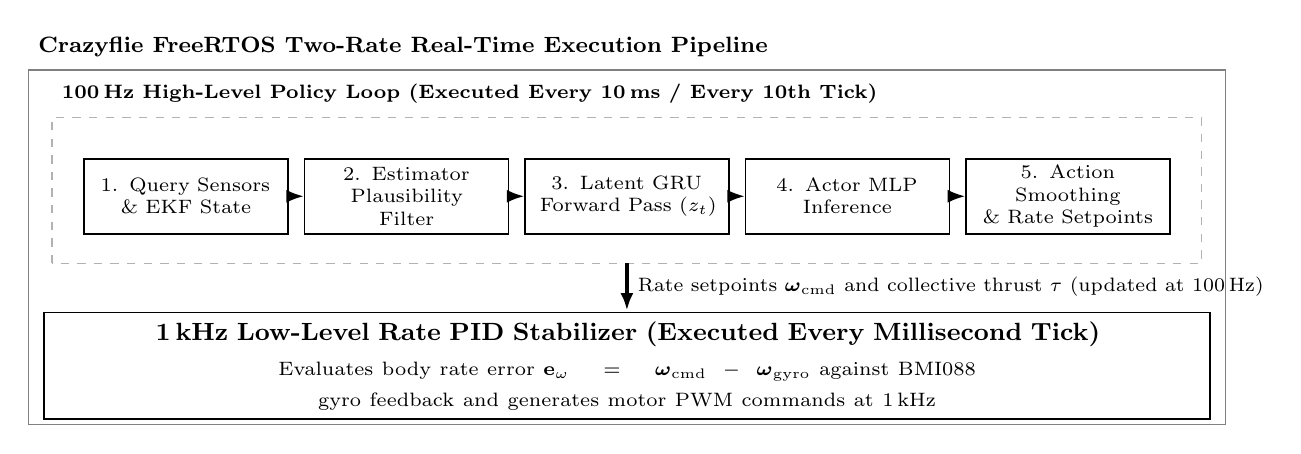
\begin{tikzpicture}[
    rblock/.style={rectangle, draw=black, line width=0.6pt, fill=white, text width=2.45cm, align=center, minimum height=0.95cm, font=\scriptsize, inner sep=2pt},
    pblock/.style={rectangle, draw=black, line width=0.6pt, fill=white, text width=14.6cm, minimum height=1.35cm, align=center, font=\small, inner sep=3pt},
    harrow/.style={-{Latex[length=2.2mm]}, thick, black}
  ]
    % Outer Frame
    \node[font=\footnotesize\bfseries, anchor=south west] at (-7.6, 2.05) {Crazyflie FreeRTOS Two-Rate Real-Time Execution Pipeline};
    \draw[draw=black!50, line width=0.6pt] (-7.6, -2.5) rectangle (7.6, 2.0);

    % 100 Hz Policy Loop Section
    \node[font=\scriptsize\bfseries, anchor=south west] at (-7.3, 1.45) {100\,Hz High-Level Policy Loop (Executed Every 10\,ms / Every 10th Tick)};
    \draw[draw=black!30, dashed, line width=0.5pt] (-7.3, -0.45) rectangle (7.3, 1.4);

    \node[rblock] (f1) at (-5.6, 0.4) {1. Query Sensors\\ \& EKF State};
    \node[rblock] (f2) at (-2.8, 0.4) {2. Estimator Plausibility\\ Filter};
    \node[rblock] (f3) at (0.0, 0.4) {3. Latent GRU\\ Forward Pass ($z_t$)};
    \node[rblock] (f4) at (2.8, 0.4) {4. Actor MLP\\ Inference};
    \node[rblock] (f5) at (5.6, 0.4) {5. Action Smoothing\\ \& Rate Setpoints};

    \draw[harrow] (f1) -- (f2);
    \draw[harrow] (f2) -- (f3);
    \draw[harrow] (f3) -- (f4);
    \draw[harrow] (f4) -- (f5);

    % Arrow down to 1 kHz loop
    \draw[harrow, very thick] (0, -0.45) -- node[right, font=\scriptsize] {Rate setpoints $\boldsymbol{\omega}_{\text{cmd}}$ and collective thrust $\tau$ (updated at 100\,Hz)} (0, -1.05);

    % 1 kHz PID Loop Section
    \node[pblock] (loop1k) at (0, -1.75) {
      \textbf{1\,kHz Low-Level Rate PID Stabilizer (Executed Every Millisecond Tick)}\\[0.2em]
      \scriptsize Evaluates body rate error $\mathbf{e}_\omega = \boldsymbol{\omega}_{\text{cmd}} - \boldsymbol{\omega}_{\text{gyro}}$ against BMI088 gyro feedback and generates motor PWM commands at 1\,kHz
    };
  \end{tikzpicture}
  \caption{Embedded FreeRTOS execution hierarchy. The neural policy runs every 10\,ms to produce rate setpoints, feeding the native 1\,kHz PID rate stabilizer on every millisecond tick.}
  \label{fig:freertos_timing}
\end{figure}

The execution pipeline follows a strict two-rate hierarchy, as illustrated in Figure~\ref{fig:freertos_timing}:
\begin{itemize}[leftmargin=*,itemsep=2pt]
  \item High-level policy loop at 100\,Hz: executes every tenth tick of the system clock. It samples the state estimate and IMU, validates data through the plausibility filter, updates the GRU latent vector, evaluates the actor MLP, and applies exponential smoothing to the commanded rates.
  \item Low-level actuator loop at 1\,kHz: executes on every millisecond tick. It compares commanded angular rates with high-rate gyroscope feedback and runs the native PID rate stabilizer to produce motor PWM signals.
\end{itemize}

\subsection{Microcontroller Resource Budget}
The trained neural networks were converted to ONNX and compiled into optimized C arrays using the ST Edge AI compiler. Inference latency measured under 0.38\,ms, using less than 4 percent of the 10\,ms time budget available at 100\,Hz.

\begin{table}[h!]
  \centering
  \small
  \caption{STM32F405 microcontroller resource utilization.}
  \label{tab:mcu_budget}
  \begin{tabularx}{\textwidth}{Xcccc}
    \toprule
    Subsystem / Resource & Allocated & Available & Utilization & Operational Margin \\
    \midrule
    Flash Memory & 596\,KB & 1,024\,KB & 58\% & More than 400\,KB free \\
    SRAM Memory & 108\,KB & 192\,KB & 83\% & 20\,KB stack headroom \\
    Execution Time per Step & 0.38\,ms & 10.00\,ms & 3.8\% & 9.62\,ms idle budget \\
    \bottomrule
  \end{tabularx}
\end{table}

Table~\ref{tab:mcu_budget} summarizes the microcontroller memory and compute consumption, confirming that the policy executes comfortably within hardware limits.

\subsection{Firmware Precautions and Crash Prevention}
Hardware flight tests indicated that optical tracking dropouts during rapid rotations can cause the extended Kalman filter to output sudden unphysical position jumps. To protect the drone during physical testing, we took practical firmware precautions that occasionally save the drone from crashing during aggressive maneuvers:

The Estimator Plausibility Filter monitors state innovations on every execution tick. It checks position changes, linear velocity increments, and total distance from the launch origin against physical flight boundaries. If an anomalous jump or complete optical packet loss occurs, the filter engages a hold mode: it freezes the policy state inputs at the last plausible estimate and temporarily suspends altitude safety aborts. This prevents false sensor readings from cutting motor throttle during inverted flight.

The Controlled Descent Failsafe engages if an unrecoverable flight error occurs, such as unexpected tilt outside an active flip window. Rather than performing a hard motor disarm, which causes the drone to fall ballistically, the failsafe switches the vehicle to self-leveling attitude mode with zero roll and pitch. It ramps collective thrust smoothly from hover level to zero over 1.2 seconds, with touchdown debouncing before final motor cutoff.

Ground station communication over 2.4\,GHz radio using a Crazyradio PA USB dongle (Figure~\ref{fig:hardware_platform}c) is kept intentionally simple. The radio link transmits basic start triggers and logs telemetry packets for offline post-flight inspection without participating in the real-time control loop.

% ==============================================================================
% SECTION 7: EXPERIMENTAL RESULTS
% ==============================================================================
\section{Experimental Results and Flight Testing}
\label{sec:results}

\subsection{Simulation Benchmark Performance}
The trained policy was benchmarked across all seven manoeuvre families in both nominal simulation and under full domain randomization over 1,000 evaluation episodes per family.

\begin{table}[h!]
  \centering
  \small
  \caption{Trajectory tracking benchmark performance across manoeuvre families.}
  \label{tab:benchmark_metrics}
  \begin{tabularx}{\textwidth}{Xcccc}
    \toprule
    Manoeuvre Family & Nominal (\%) & Robust DR (\%) & Peak Speed (m/s) & Completion (\%) \\
    \midrule
    Precision Hover & 79.2 & 76.5 & 0.12 & 100.0\% \\
    3D Polynomial Waypoints & 85.4 & 81.2 & 1.85 & 99.8\% \\
    Lemniscate Figure-8 & 83.1 & 79.4 & 1.62 & 99.5\% \\
    Vertical Figure-8 & 93.2 & 88.6 & 2.45 & 98.9\% \\
    Slalom Weave & 90.5 & 85.3 & 2.10 & 99.2\% \\
    3D Orbit & 83.7 & 80.1 & 1.45 & 100.0\% \\
    Lissajous Curves & 83.0 & 78.9 & 1.55 & 99.4\% \\
    360° Power Flip & 91.0 & 84.7 & 3.22 & 97.4\% \\
    \midrule
    Composite Average & 85.0\% & 81.8\% & --- & 99.3\% \\
    \bottomrule
  \end{tabularx}
\end{table}

As summarized in Table~\ref{tab:benchmark_metrics}, the controller achieves an 85.0 percent composite tracking score across all trajectories, maintaining completion rates above 97 percent even during aggressive vertical manoeuvres and flips.

\begin{figure}[t!]
  \centering
  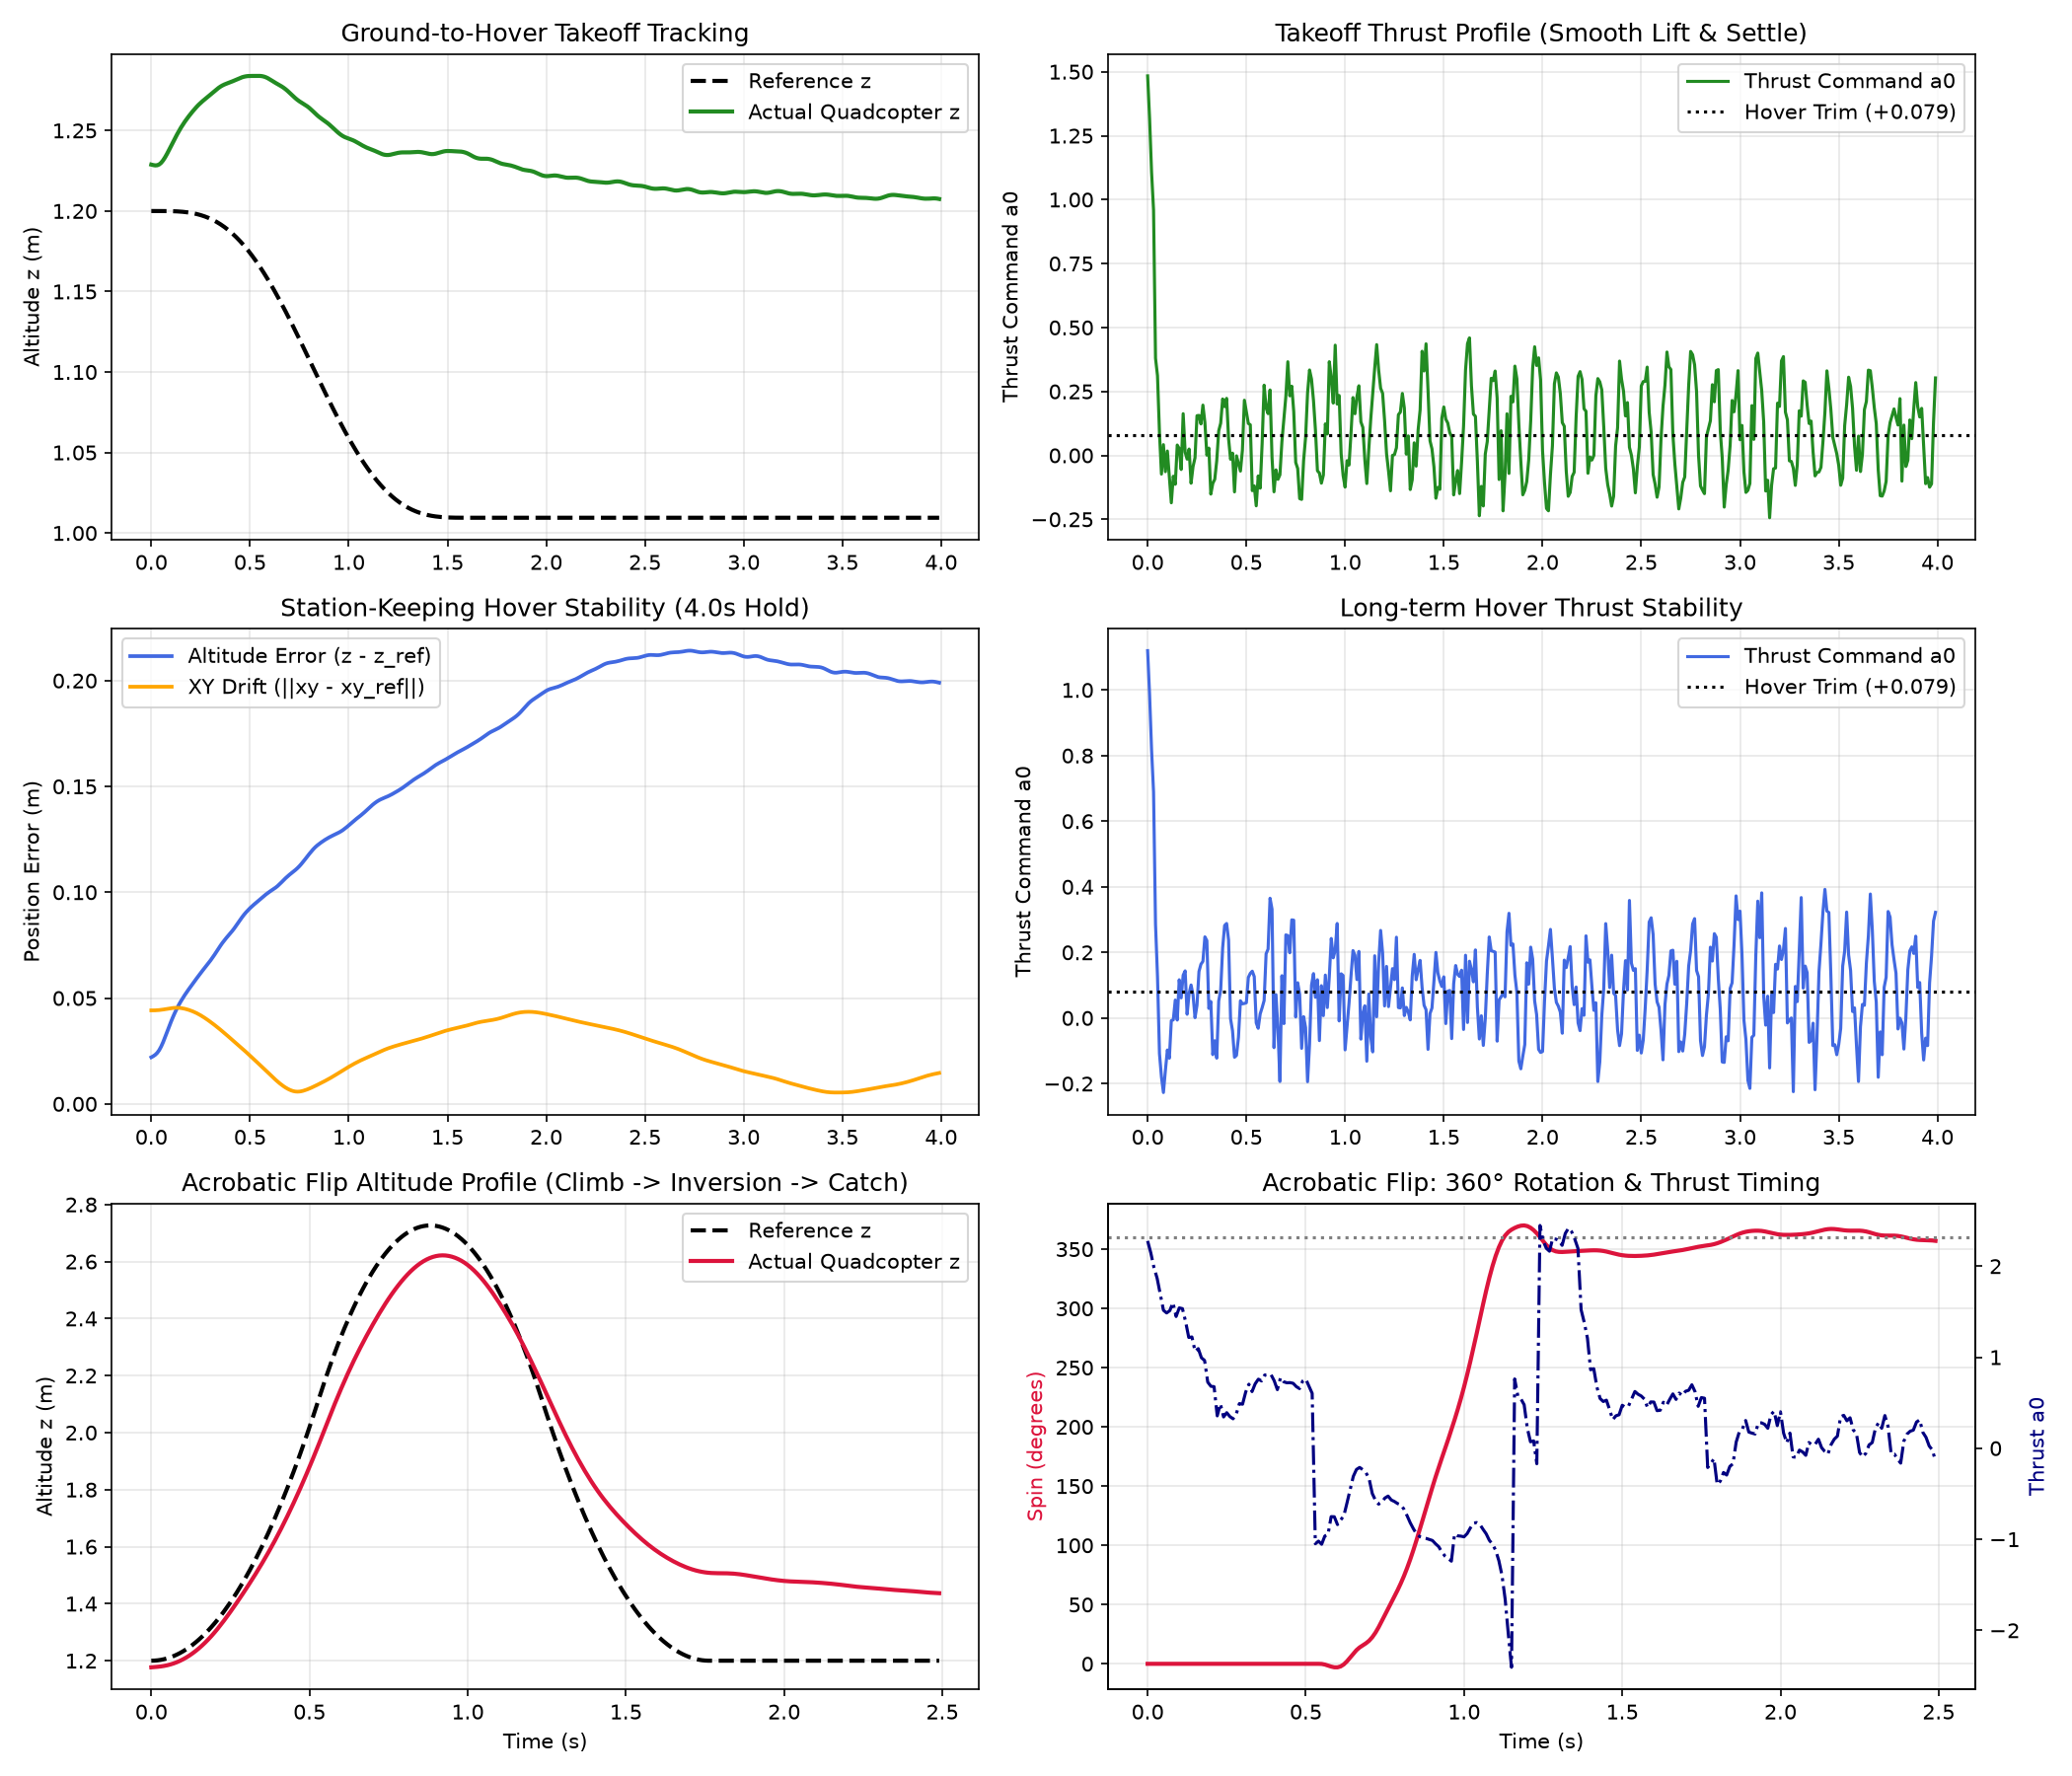
\includegraphics[width=0.82\textwidth]{figures/flight_trajectories_mjx.png}
  \caption{Simulation tracking performance in MuJoCo MJX. Top row shows takeoff altitude tracking and thrust command settling. Middle row presents station-keeping hover stability over extended holds. Bottom row demonstrates the acrobatic flip altitude profile and rotation angle progression.}
  \label{fig:flight_trajectories}
\end{figure}

Figure~\ref{fig:flight_trajectories} shows simulation traces of takeoff tracking, station-keeping hover hold, and the altitude and rotation dynamics of an acrobatic flip. Figure~\ref{fig:training_curves} illustrates policy learning progress during 30 million training steps in MuJoCo MJX, including reward curves, evaluation scores across manoeuvres, optimization loss terms, and curriculum scheduling.

\begin{figure}[t!]
  \centering
  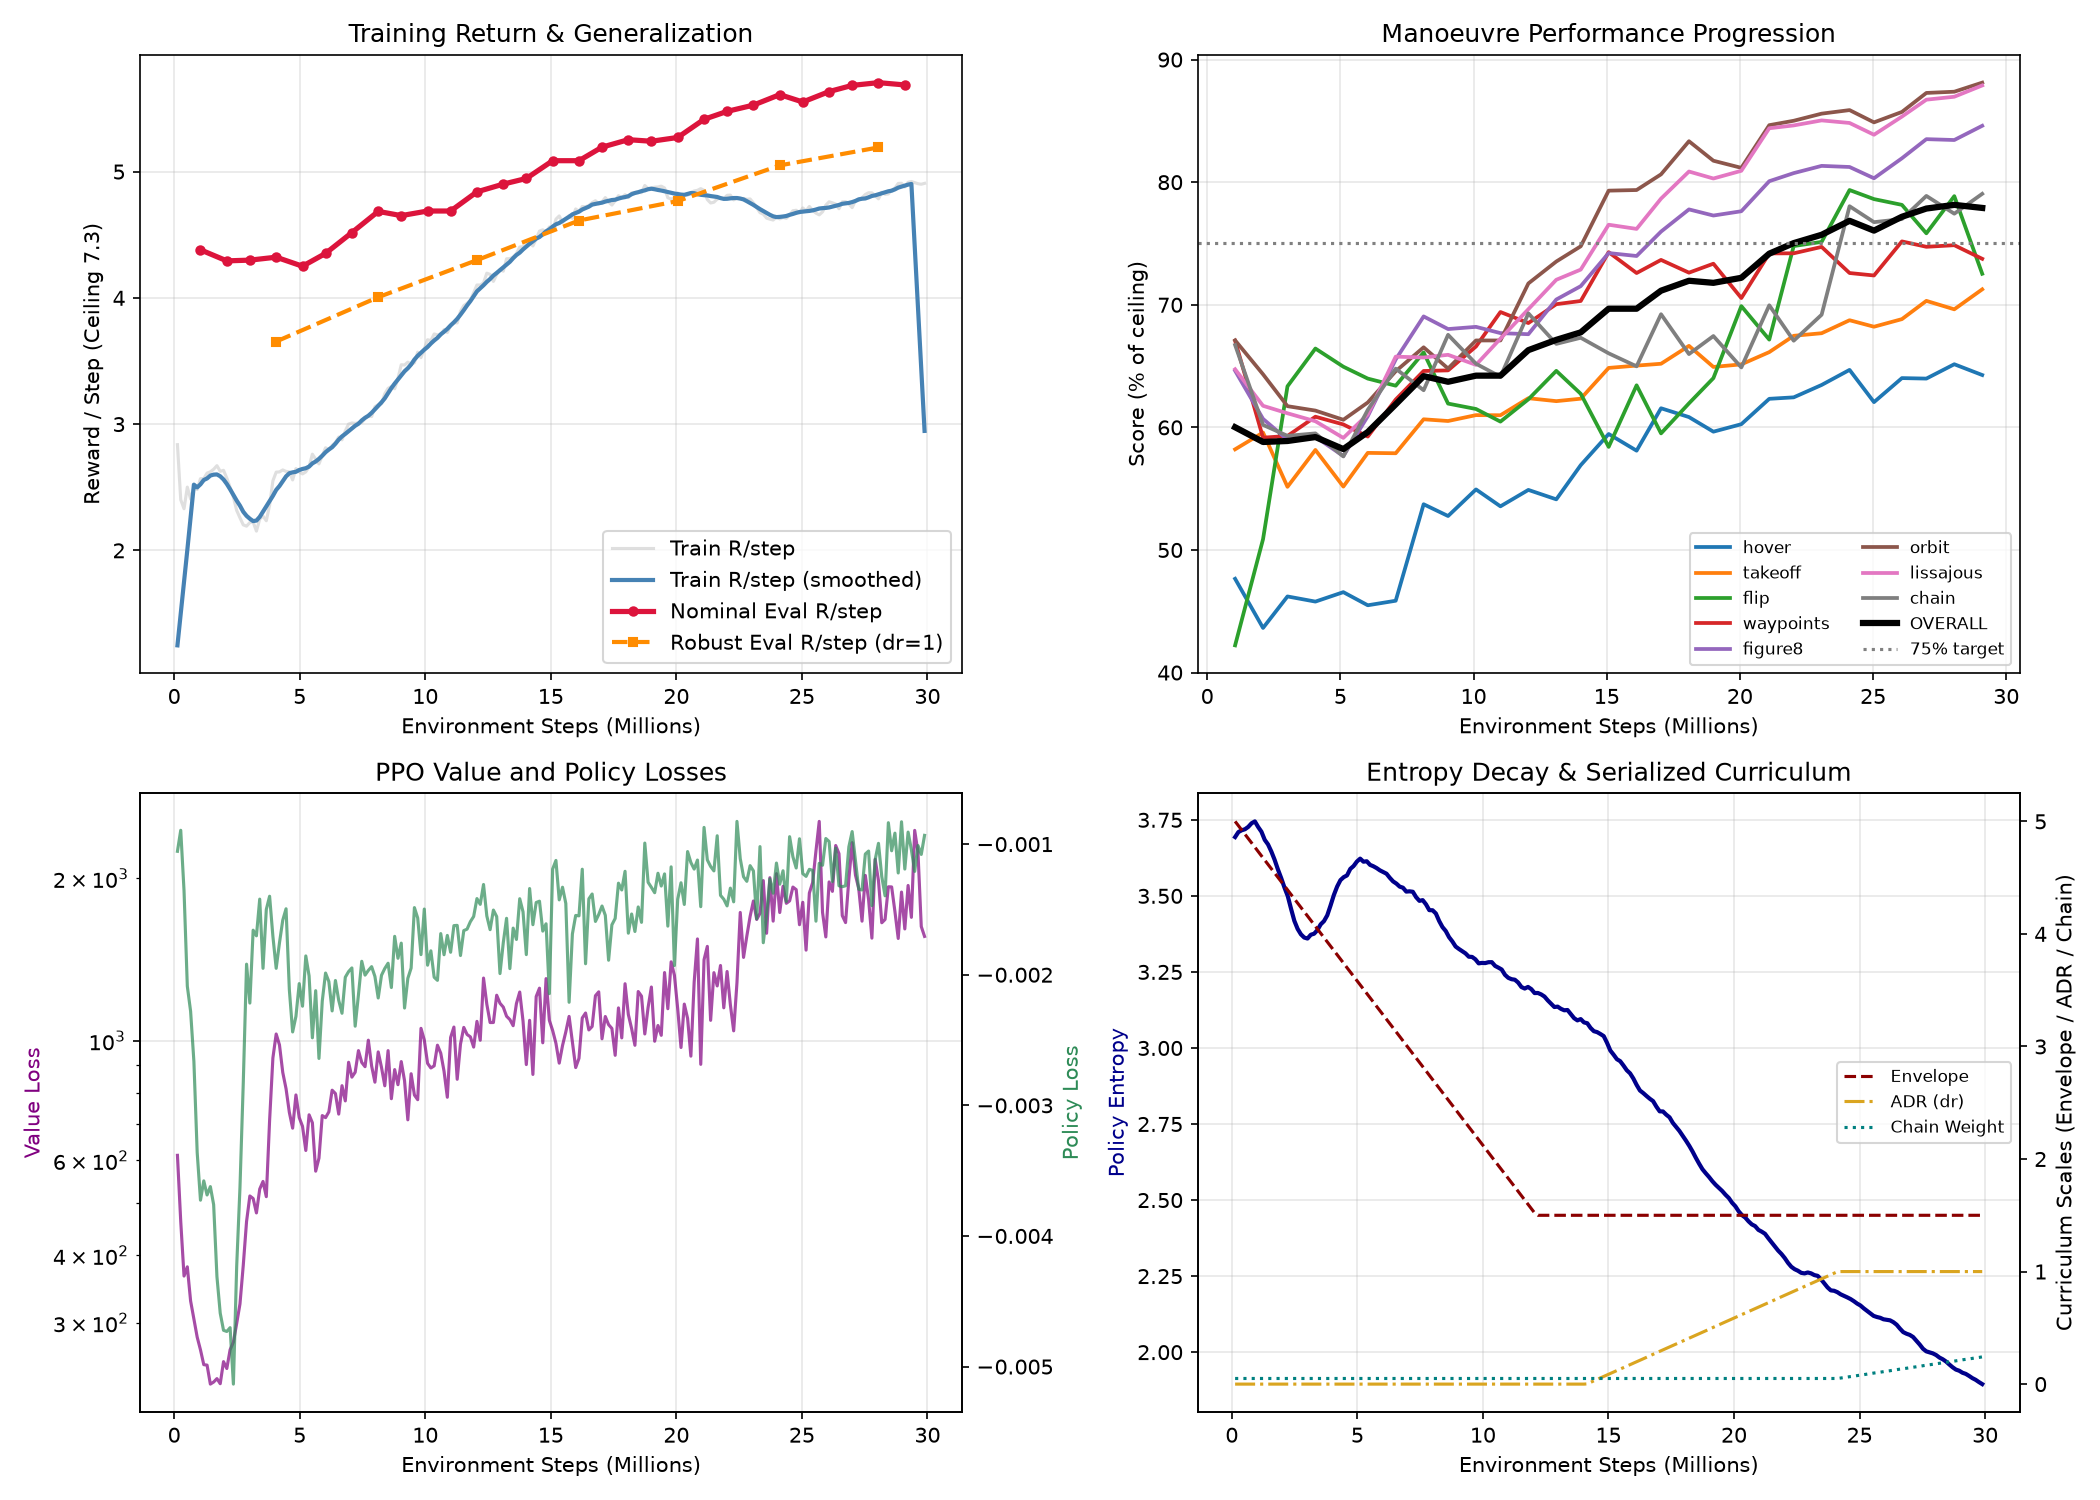
\includegraphics[width=0.80\textwidth]{figures/training_curves_mjx.png}
  \caption{Reinforcement learning training progress in MuJoCo MJX. Subplots show training reward progression, manoeuvre evaluation scores, PPO value and policy losses, and policy entropy decay alongside domain randomization curriculum progression over 30 million timesteps.}
  \label{fig:training_curves}
\end{figure}

\subsection{Physical Hardware Flight Demonstration}
The trained policy was flashed onto the physical Crazyflie 2.1 and validated inside an indoor flight space equipped with Lighthouse v2 positioning. Telemetry packets were recorded over radio at 100\,Hz.

\begin{figure}[t!]
  \centering
  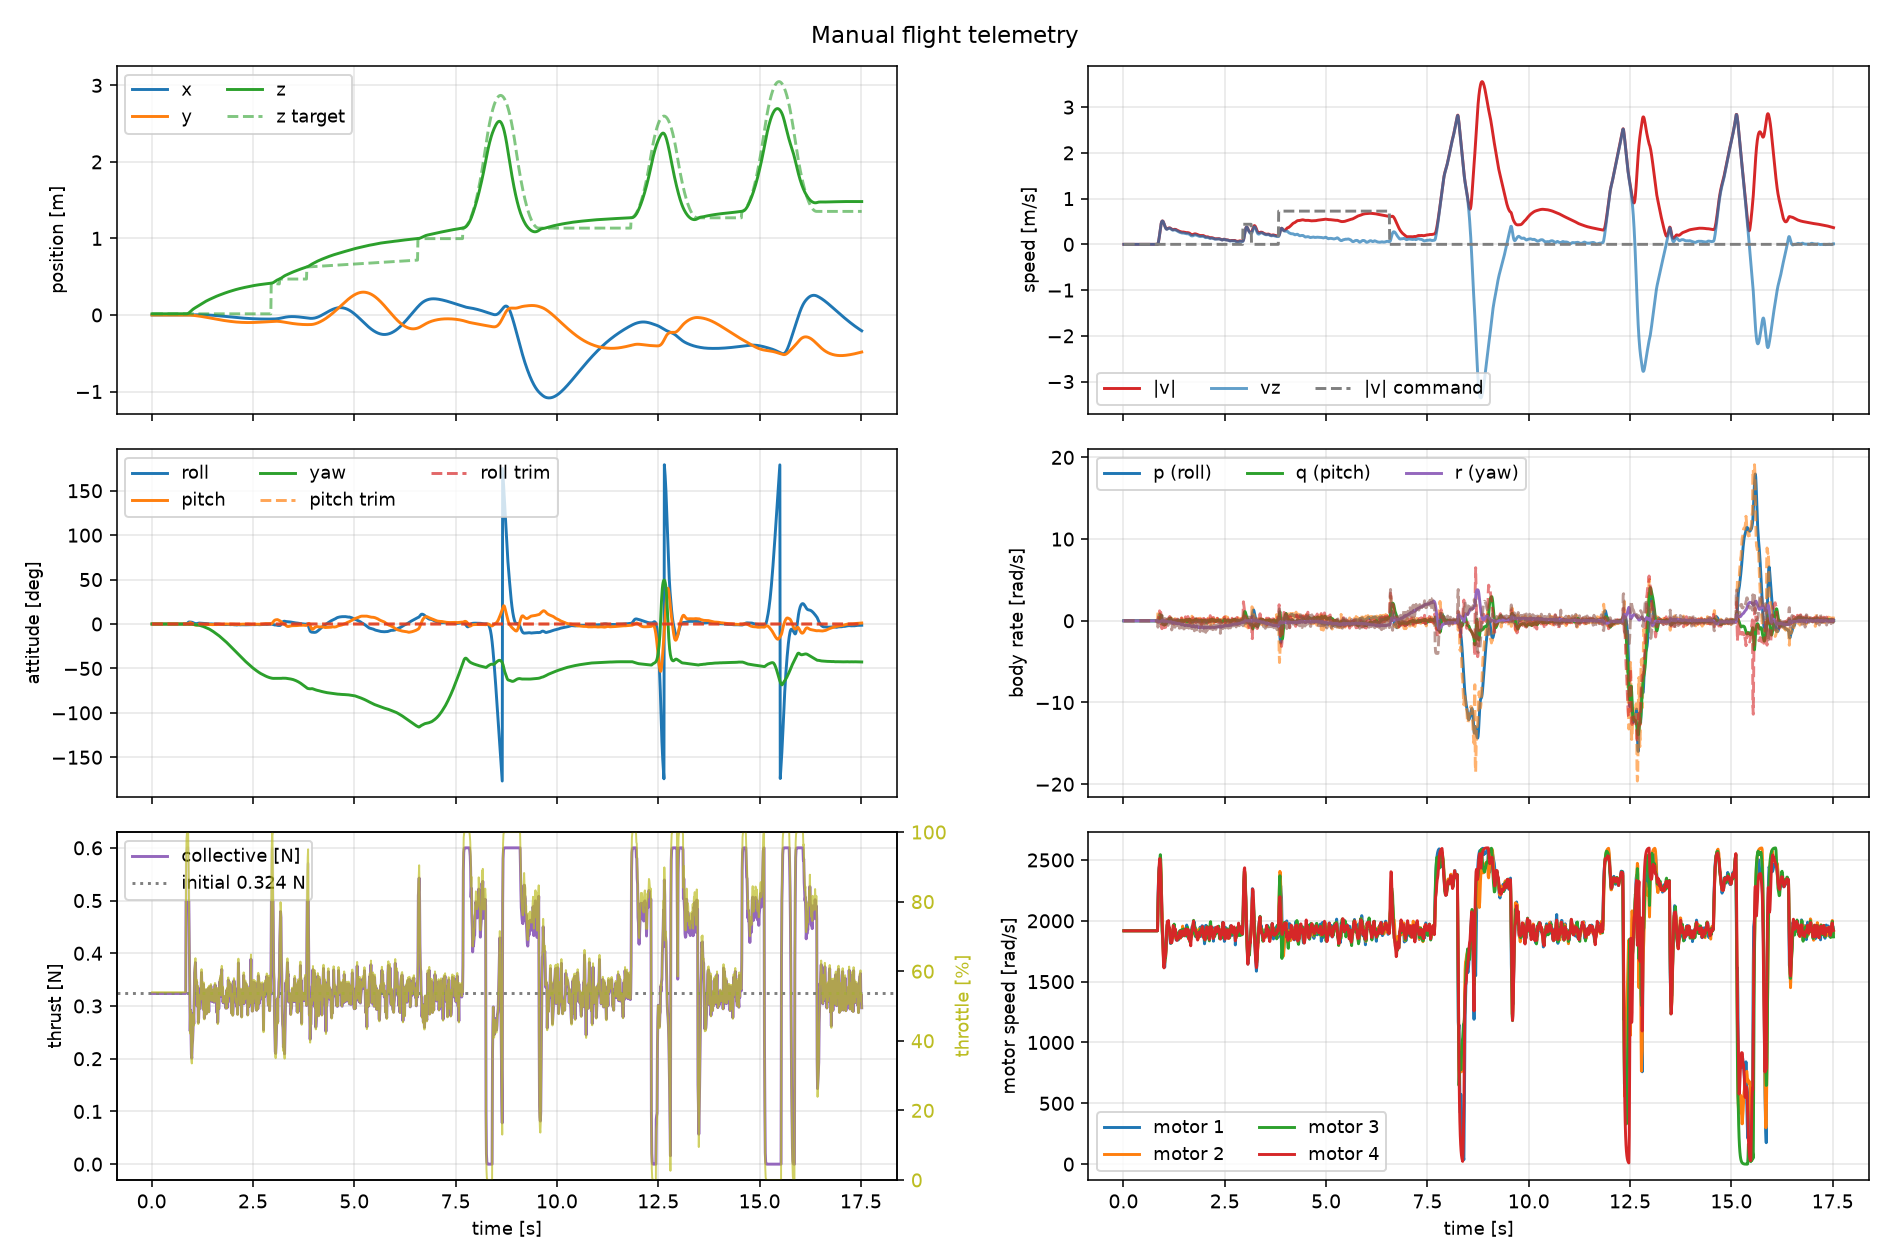
\includegraphics[width=0.84\textwidth]{figures/live_flight_telemetry.png}
  \caption{Hardware flight telemetry recorded during physical testing. Top row displays 3D position coordinates and linear velocity. Middle row shows roll, pitch, and yaw attitude angles along with body angular rates. Bottom row presents collective thrust command and individual motor rotational speeds.}
  \label{fig:live_telemetry}
\end{figure}

The physical flight tests demonstrated successful autonomous completion of 360-degree flips without manual intervention. During the flip manoeuvre:
\begin{itemize}[leftmargin=*,itemsep=2pt]
  \item The quadcopter initiated the climb pop, applying saturated collective thrust to accelerate vertically and establish clearance.
  \item The policy commanded high body rates to rotate through full inversion while reducing collective thrust to coast ballistically, preventing the vehicle from driving downward.
  \item During inversion, optical reception dropped as top-mounted photodiodes lost line of sight to the base stations. The plausibility filter successfully held state estimates, preventing false altitude spikes from triggering an abort.
  \item Upon completing rotation, counter-torque halted the angular motion and thrust ramped up to arrest descent, bringing the vehicle back to an upright hover.
\end{itemize}

Figure~\ref{fig:live_telemetry} presents the recorded telemetry from these flight experiments, showing synchronized position, attitude angles, body rates, collective thrust, and individual motor speeds.

\subsection{Inner-Loop Rate Tracking Response}
Figure~\ref{fig:rate_tracking} illustrates the inner-loop rate PID tracking performance during physical flight. Commanded angular rates from the neural policy are tracked closely by the onboard 1\,kHz rate controller, confirming minimal phase delay across roll, pitch, and yaw axes.

\begin{figure}[t!]
  \centering
  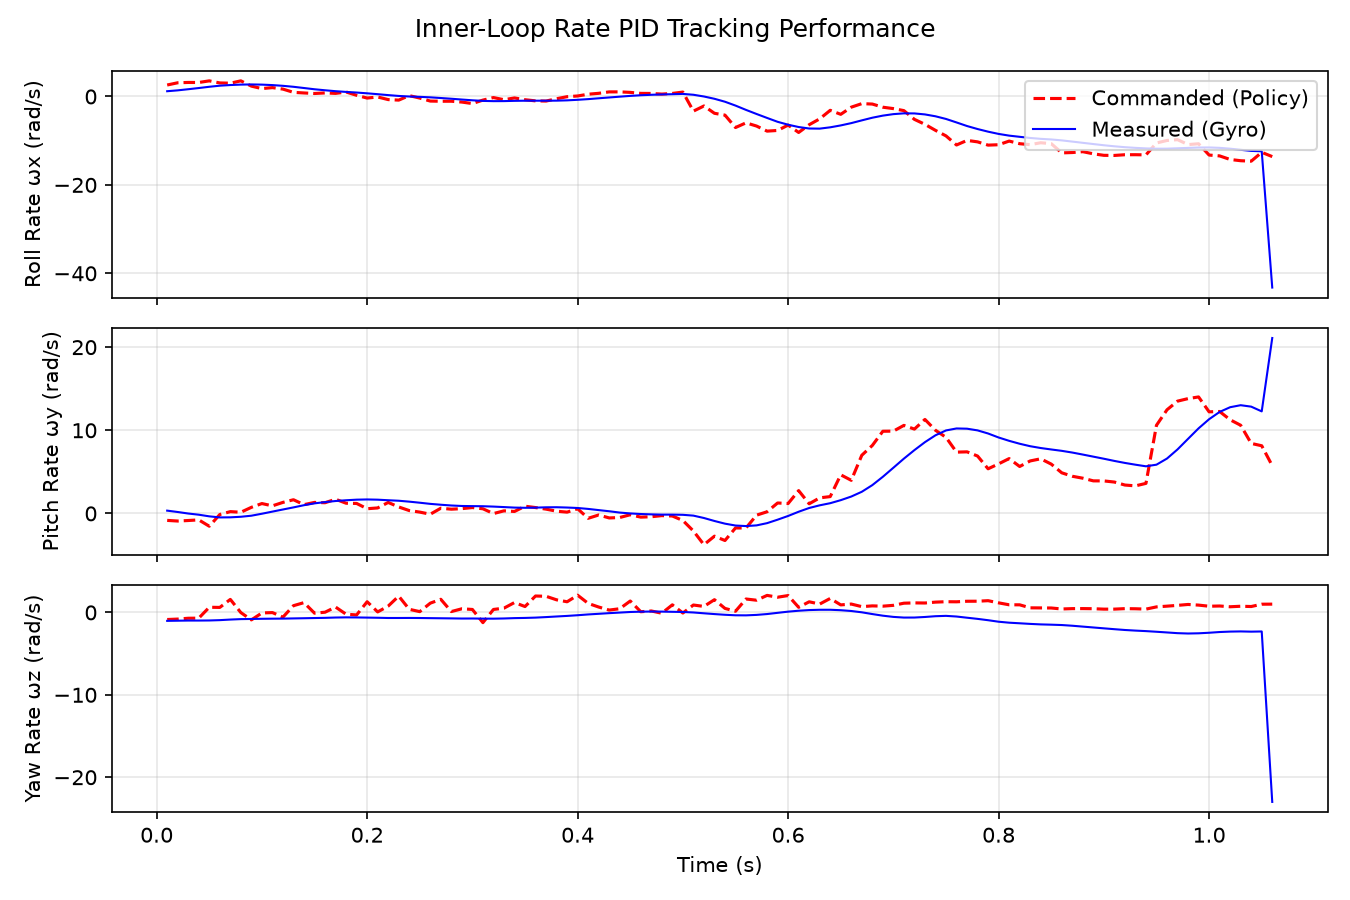
\includegraphics[width=0.55\textwidth,height=3.8cm,keepaspectratio]{figures/rate_tracking_plot.png}
  \vspace{-0.3em}
  \caption{Onboard 1\,kHz rate PID tracking performance. Commanded rate setpoints from the policy are closely tracked by measured gyroscope feedback, confirming responsive inner-loop control.}
  \label{fig:rate_tracking}
\end{figure}

% ==============================================================================
% SECTION 8: PRACTICAL LESSONS & CONCLUSION
% ==============================================================================
\section{Practical Lessons and Conclusion}
\label{sec:conclusion}

\subsection{Engineering Insights}
Several practical takeaways emerged from building and flying this system:
\begin{itemize}[leftmargin=*,itemsep=2pt]
  \item Body rate control is essential for aerobatics. Inversion cannot be commanded through tilt-angle interfaces because self-leveling modes fight rotation past 90 degrees. Direct rate setpoints feeding a 1\,kHz inner stabilizer provide reliable control authority.
  \item Recurrent latent representations provide effective sim-to-real transfer. By encoding temporal sensor sequences into a compact latent vector, the policy adapts to battery discharge and motor hardware variations without retraining.
  \item Firmware-level plausibility checks are required when deploying learning-based policies. Learned models cannot compensate for corrupt sensor inputs, making lightweight safety filters in firmware indispensable during aggressive flight.
\end{itemize}

\subsection{Conclusion}
This project demonstrates that deep reinforcement learning, combined with asymmetric training and recurrent latent history encoding, enables agile aerobatic manoeuvres on micro quadcopters with strict compute and payload constraints. By pairing high-throughput parallel simulation in MuJoCo MJX with bare-metal C deployment through ST Edge AI on FreeRTOS, the complete control pipeline runs on an ARM Cortex-M4 microcontroller, achieving autonomous acrobatic flips directly onboard a physical quadcopter.

% ==============================================================================
% REFERENCES
% ==============================================================================
\begin{thebibliography}{99}
\footnotesize
\setlength{\itemsep}{0pt}
\setlength{\parskip}{0pt}
\bibitem{kaufmann2023champion}
E.~Kaufmann, L.~Bauersfeld, A.~Loquercio, M.~M{\"u}ller, V.~Koltun, and D.~Scaramuzza, ``Champion-level drone racing using deep reinforcement learning,'' \emph{Nature}, vol. 620, no. 7976, pp. 982--987, 2023.

\bibitem{foehn2021alphapilot}
P.~Foehn, A.~Romero, and D.~Scaramuzza, ``Time-optimal planning for quadrotors with cable-suspended payloads,'' \emph{IEEE Robotics and Automation Letters}, vol. 6, no. 2, pp. 1625--1632, 2021.

\bibitem{hwangbo2019control}
J.~Hwangbo, J.~Lee, A.~Dosovitskiy, D.~Mellinger, K.~Kalyan, and M.~Hutter, ``Learning agile and dynamic motor skills for legged robots,'' \emph{Science Robotics}, vol. 4, no. 26, p. eaau5872, 2019.

\bibitem{schulman2017proximal}
J.~Schulman, F.~Wolski, P.~Dhariwal, A.~Radford, and O.~Klimov, ``Proximal policy optimization algorithms,'' \emph{arXiv preprint arXiv:1707.06347}, 2017.

\bibitem{todorov2012mujoco}
E.~Todorov, T.~Erez, and Y.~Tassa, ``MuJoCo: A physics engine for model-based control,'' in \emph{IEEE/RSJ International Conference on Intelligent Robots and Systems (IROS)}, 2012, pp. 5026--5033.

\bibitem{pinto2021asymmetric}
L.~Pinto, M.~Andrychowicz, P.~Welinder, W.~Zaremba, and P.~Abbeel, ``Asymmetric actor critic for image-based robot learning,'' \emph{Robotics: Science and Systems (RSS)}, 2018.

\bibitem{mellinger2011minimum}
D.~Mellinger and V.~Kumar, ``Minimum snap trajectory generation and control for quadrotors,'' in \emph{IEEE International Conference on Robotics and Automation (ICRA)}, 2011, pp. 2520--2525.

\bibitem{bitcraze2026}
Bitcraze AB, ``Crazyflie 2.1 open-source nano-quadcopter platform,'' \url{https://www.bitcraze.io/products/crazyflie-2-1/}, 2026.
\end{thebibliography}

% ==============================================================================
% APPENDIX
% ==============================================================================
\newpage
\appendix
\section*{Appendix: Technical Specifications and Hyperparameters}
\label{sec:appendix}

\begin{table}[h!]
  \centering
  \small
  \caption{Actor and critic observation vector specifications.}
  \label{tab:obs_spec}
  \begin{tabularx}{\textwidth}{lp{4.2cm}ccX}
    \toprule
    Indices & Observation Field & Dim & Units & Description \\
    \midrule
    \multicolumn{5}{l}{\textit{Deployable Actor Observation Vector (Total: 48 Dimensions)}} \\
    0 -- 2 & Estimated Position & 3 & m & Position estimate from optical EKF \\
    3 -- 6 & Attitude Quaternion & 4 & --- & Unit quaternion $[q_w, q_x, q_y, q_z]^T$ \\
    7 -- 9 & Body Angular Rates & 3 & rad/s & Filtered angular velocity from IMU \\
    10 -- 11 & Linear Velocity XY & 2 & m/s & Estimated horizontal velocity \\
    12 & Linear Velocity Z & 1 & m/s & Estimated vertical climb rate \\
    13 -- 16 & Previous Action & 4 & $[-1, 1]$ & Low-pass filtered control effort history \\
    17 -- 19 & Position Error & 3 & m & $\mathbf{p}_{\text{ref}} - \hat{\mathbf{p}}$ \\
    20 -- 22 & Velocity Error & 3 & m/s & $\mathbf{v}_{\text{ref}} - \hat{\mathbf{v}}$ \\
    23 -- 25 & Attitude Error & 3 & --- & Vector component of $\mathbf{q}_{\text{ref}}^* \otimes \mathbf{q}$ \\
    26 -- 28 & Angular Rate Error & 3 & rad/s & $\boldsymbol{\omega}_{\text{ref}} - \boldsymbol{\omega}$ \\
    29 -- 44 & Latent Representation & 16 & --- & Implicit feature vector from GRU \\
    45 -- 47 & Feedforward Reference & 3 & m/s & Trajectory target feedforward velocity \\
    \midrule
    \multicolumn{5}{l}{\textit{Privileged Critic Observation Vector (Total: 96 Dimensions)}} \\
    0 -- 47 & Deployable Actor Frame & 48 & mixed & Exact inputs seen by the actor policy \\
    48 -- 50 & Ground Truth Position & 3 & m & True simulation position \\
    51 -- 53 & Ground Truth Velocity & 3 & m/s & True linear velocity without sensor delay \\
    54 -- 57 & Ground Truth Quaternion & 4 & --- & True attitude quaternion without noise \\
    58 -- 61 & Rotor Speeds & 4 & rad/s & Motor rotational speeds \\
    62 -- 64 & Aerodynamic Drag Vector & 3 & N & Body aerodynamic drag forces \\
    65 & Thrust Degradation Factor & 1 & --- & Battery sag scaling factor \\
    66 -- 69 & Motor Time Constants & 4 & s & Actual simulated ESC time constants \\
    70 -- 95 & Disturbance and Sensor States & 26 & mixed & Wind vectors, sensor noise, delay states \\
    \bottomrule
  \end{tabularx}
\end{table}

\begin{table}[h!]
  \centering
  \small
  \caption{Proximal Policy Optimization hyperparameters.}
  \label{tab:ppo_hyperparams}
  \begin{tabularx}{\textwidth}{lX}
    \toprule
    Hyperparameter Parameter & Configured Value \\
    \midrule
    Parallel Rollout Environments in MJX & 1,024 environments \\
    Rollout Steps per Iteration & 128 steps \\
    Minibatch Size & 2,048 \\
    Optimization Epochs per Iteration & 4 epochs \\
    Discount Factor ($\gamma$) & 0.99 \\
    Generalized Advantage Estimation ($\lambda_{\text{GAE}}$) & 0.95 \\
    PPO Clip Parameter ($\epsilon$) & 0.20 \\
    Actor Learning Rate (Linear Decay) & $3.0 \times 10^{-4} \to 1.0 \times 10^{-5}$ \\
    Critic Learning Rate & $1.0 \times 10^{-3} \to 5.0 \times 10^{-5}$ \\
    Entropy Regularization Coefficient & $0.01 \to 0.001$ \\
    Optimizer & Adam ($\beta_1=0.9, \beta_2=0.999, \epsilon=10^{-8}$) \\
    Action Moving Average Smoothing ($\alpha$) & 0.80 \\
    Total Training Timesteps & 30,000,000 steps (3.58 hours) \\
    \bottomrule
  \end{tabularx}
\end{table}

\end{document}
